\documentclass[conference]{IEEEtran}
\IEEEoverridecommandlockouts

\usepackage{tikz}
\usepackage{amsmath}
\usepackage{amssymb,amsfonts} 
\usepackage{algorithmic}
\usepackage{graphicx}
\usepackage{textcomp}
\usepackage{xcolor}
\usepackage{verbatim}
\usepackage{caption}
\usepackage{url}
\usepackage{subcaption}
\usepackage{subfig}


\usepackage{wrapfig,lipsum,booktabs}
% \usepackage[inkscapeformat=png]{svg}
\usepackage{svg}
% \usepackage{svg}
\usepackage{tikz}
\usepackage{makecell}

\usepackage{colortbl}
\usepackage{booktabs}
\usepackage{multirow}
\usepackage{float}
\usepackage[table]{xcolor}
\usepackage{pgf}

\usepackage{adjustbox}
\usepackage{boldline}
\usepackage{caption}
\usepackage{listings}
\usepackage{eqnarray}
\usepackage{xurl} 




%-------------------------------------------------------------------------------
%\hyphenation{OptiMAC, vulnerability}

\begin{document}
%-------------------------------------------------------------------------------

%don't want date printed
\date{}

% make title bold and 14 pt font (Latex default is non-bold, 16 pt)
\title{\Large \bf OptiMAC: Adaptive Security Optimization for \\Message Authentication Code in Adversarial Environment}

%for single author (just remove % characters)
% \author{
% {\rm SeyedMohammad Kashani}\\
% Iowa State University
% \and
% {\rm Erfan Khademnia}\\
% Iowa State University
% \and
% {\rm G\"{o}rkem Emirh\"{u}seyino\u{g}lu}\\
% Iowa State University
% \and
% {\rm Yilu Dong}\\
% Pennsylvania State University
% \and
% {\rm Tianwei Wu}\\
% Pennsylvania State University
% \and
% {\rm Farid Nait-Abdesselam}\\
% Universit\'e Paris Cit\'e
% \and
% {\rm Ashfaq Khokhar}\\
% Iowa State University
% \and
% {\rm Sang W. Kim}\\
% Iowa State University
% \and
% {\rm Syed Hussain Rafiul}\\
% Pennsylvania State University
% } % end author

 \author{\IEEEauthorblockN{SeyedMohammad Kashani\IEEEauthorrefmark{1},
		 Erfan Khademnia\IEEEauthorrefmark{2},
		 G\"{o}rkem Emirh\"{u}seyino\u{g}lu\IEEEauthorrefmark{2}, 
		 Yilu Dong\IEEEauthorrefmark{3},
		 Tianwei Wu\IEEEauthorrefmark{3},\\
		 Sang Wu Kim\IEEEauthorrefmark{1},
		 Ashfaq Khokhar\IEEEauthorrefmark{1},
		 Farid Nait-Abdesselam\IEEEauthorrefmark{4},
		 and Syed Hussain Rafiul\IEEEauthorrefmark{3}, 
		 }
	 \IEEEauthorblockA{\IEEEauthorrefmark{1}Department of Electrical and Computer Engineering,
		 Iowa State University}
	 \IEEEauthorblockA{\IEEEauthorrefmark{2} Industrial and Manufacturing Systems Engineering, Iowa State University\\
		 \IEEEauthorblockA{\IEEEauthorrefmark{3}School of Electrical Engineering and Computer Science, Pennsylvania State University}
		 \IEEEauthorblockA{\IEEEauthorrefmark{4}Laboratory of Informatics at Paris Descartes, Université Paris Cité}
		 \IEEEauthorrefmark{1} \{kashani,swkim, ashfaq\}@iastate.edu,
		 \IEEEauthorrefmark{2} \{gorkem, erfank\}@iastate.edu
		 \IEEEauthorrefmark{3} \{yiludong,tvw5452,hussain1\}@psu.edu}
	 \IEEEauthorrefmark{4} \
	 {farid.nait-abdesselam@u-paris.fr}}
	
	
\maketitle
\begingroup\renewcommand\thefootnote{\textsection}



\maketitle

%-------------------------------------------------------------------------------
\begin{abstract}
% Integrity verification methods using Message Authentication Codes (MAC) often impose significant computational and bandwidth overhead. While the short MAC was initially proposed to reduce this overhead, it compromises security. Alternative schemes, such as aggregate, compound, and progressive MACs, have been developed to maintain security levels while reducing overhead and computational demands. However, these heuristic methods remain susceptible to Denial of Service (DoS) and jamming attacks, particularly in critical wireless environments. This paper develops a new optimization framework for integrity mechanism that is based on a novel mapping of the problem to a graph, allowing for the deployment of mathematical optimizations. OptiMAC maximizes the expected number of tag bits per message, ensuring optimal security measures for integrity check system under adversarial scenarios. This is achieved by our novel unifying framework and innovative metrics to represent security and efficiency, enabling the optimization model to identify optimal message-tag assignments. Through extensive real-world testing on live webcam video streaming over Wi-Fi and 5G, we demonstrate a constant improvement in the number of tag bits per message compared to existing methods, validating our methodology. 
% This paper presents an optimized MAC aggregation framework that enhances integrity checks in wireless communications under adversarial conditions. Building on the Progressive MAC (ProMAC) model, our approach systematically defines parameters like tag generation and update rules, allowing adaptive optimization for resilience against forgery, denial of service (DoS), and lossy channel conditions.
% Leveraging existing security proofs from ProMAC and aggregate MAC studies, our framework introduces the Strength Number (SN) metric to enhance resilience. By optimizing the tag-to-message ratio within a dependency area calculated as \(2^{n \times m}\), we create a broad solution space that improves both latency and security.
% Experimental results across varying attack rates show that higher dependency areas (e.g., a 15/30 tag-to-message ratio) outperform configurations with similar ratios (like 10/20) in terms of SN and latency. This scalable framework is particularly suited for secure, resource-constrained wireless applications, demonstrating an adaptable, efficient approach to improving MAC scheme reliability in hostile environments.
Integrity verification utilizing Message Authentication Codes (MACs) can impose high overhead by generating and transmitting extra bits. Alternatively, grouping multiple messages and sending only one MAC for the group can reduce the computational and energy expenditure. However, in such grouping scenarios, the MAC depends on the each of the messages to validate the integrity of the entire group. Therefore, even with a single message loss, the MAC becomes unusable. In adversarial wireless environments, such as under jamming, this grouping strategy can make the system vulnerable to a denial-of-service attack. To address this, we propose OptiMAC, which addresses the shortcomings of the Progressive MAC (ProMAC) framework to increase the resiliency to message losses. In the ProMAC framework, each MAC is derived from an evolving state that holds a buffer of multiple messages and is updated with every new message. While the ProMAC framework's security is proven in principle, it lacks a systematic approach to defining the optimal state update rule for varying channel quality. Our proposed OptiMAC framework (i) formulates the state update process as a message grouping optimization problem and maximizes the number of usable MACs for any jamming probability, and (ii) uses simulations to find the optimum MAC length, which further maximizes throughput. Experiments over WiFi and 5G indicate improvements in security and efficiency.

\end{abstract}

\section{Introduction}\label{Introduction}


% Ensuring data integrity is fundamental to secure communication. Without integrity check mechanisms, receivers cannot verify the authenticity of received data, leaving systems vulnerable to malicious data modification. The critical role of integrity verification has been underscored by several real-world incidents. For instance, in 2011, a U.S. drone lacking GPS integrity checks was captured after adversaries successfully hijacked it by transmitting falsified GPS signals (GPS spoofing attack)~\cite{drone_gps_spoofing}.

% To mitigate such vulnerabilities, integrity-check mechanisms are indispensable. In practice, this is most commonly realized through the Message Authentication Code (MAC), computed from the message and a secret key shared between sender and receiver. The tag is transmitted alongside the message, allowing the receiver to verify its integrity. However, generating and transmitting these additional bits introduces both communication and computational overhead, which can be especially costly in power-constrained or latency-sensitive systems.
% % \textcolor{red}{ Leading to many systems, including the Global Navigation Satellite System (GNSS), to avoid implementing integrity check mechanisms~\cite{compoundMAC}}.
% Fifth-generation (5G) network is another case in point, which leaves MAC implementation optional for mobile network operators~\cite {etsi_ts_133501_v17_5_0, 5G_criticality}. However, to reduce security risks, the integrity check implementation should be mandatory. This implies the necessity of research in reducing MAC overhead in order to maintain the performance. 


Ensuring data integrity is fundamental to secure communication. Without integrity checks, receivers cannot verify the authenticity of received data, leaving systems vulnerable to malicious modification. The critical role of integrity verification has been underscored by real-world incidents; for example, in 2011 a U.S.\ drone reportedly lacking GPS integrity checks was captured after adversaries hijacked it by transmitting falsified GPS signals (a GPS spoofing attack)~\cite{drone_gps_spoofing}. In practice, data integrity is most commonly realized via Message Authentication Codes (MACs): a short tag computed from the message using a secret key shared between sender and receiver. Transmitting and verifying MACs, however, introduces both communication and computational overhead, which is especially costly in power-constrained and latency-sensitive systems. Moreover, in the fifth-generation (5G) cellular standard, MAC deployment at certain layers is not mandatory to maintain high performance and is left optional for mobile network operators to implement~\cite{etsi_ts_133501_v17_5_0,5G_criticality}. This further motivates techniques that reduce overhead without compromising security.

% Previous efforts, such as short MAC, aggregate MAC, compound MAC ..., have aimed to decrease this overhead~\cite{ProMAC1, aggregateMAC, compoundMAC}. Nonetheless, these solutions fall short in ensuring data integrity in adversarial environments. Short MAC, as illustrated in Figure~\ref{fig:truncate}, proposes reducing the tag length to decrease the overhead, at the cost of increasing the likelihood of successful forgery~\cite{ProMAC1}. Short MAC's vulnerability was exploited to modify the packets that were transmitted to a badge reader, allowing unauthorized access to a secured building~\cite{badgeOfShame}.
% \begin{figure}[h!]
%     \centering
%     \begin{subfigure}{\columnwidth}
%     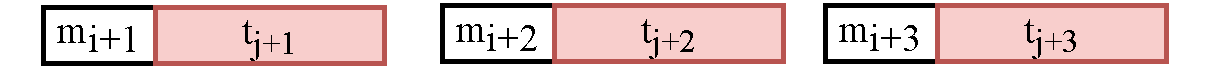
\includegraphics[width= \columnwidth]{img/MAC/TradMAC.pdf} 
%     \caption{Traditional MAC}
%         \vspace{.3cm}
%     \label{fig:traditional}
%     \end{subfigure}

%     \begin{subfigure}{\columnwidth}
%     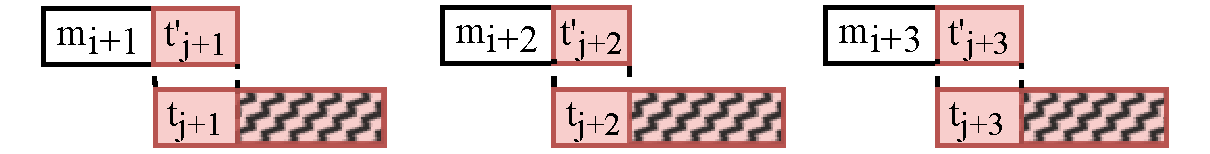
\includegraphics[width= \columnwidth]{img/MAC/TruncMAC.pdf}
%     \caption{Truncate MAC}
%     \label{fig:truncate}
%     \end{subfigure}
%     \caption{\small '$m$' represent the message and '$t$' represents the MAC (also called tag). Truncating the tag decreases the security~\cite{ProMAC1, badgeOfShame}.}
% \end{figure}

% On the other hand, aggregate and compound MACs reduce MAC overhead by verifying a group of multiple messages with only one tag~\cite{aggregateMAC, compoundMAC}. Although this approach could be effective, it is susceptible to random jamming in an adversarial wireless environment. Checking the integrity of multiple messages with one tag creates a verification dependency, where even if one of the dependent messages is lost, the whole group verification will be stopped. This is because the tag requires all of the messages in the group to be correctly received prior to performing the integrity check. Therefore, with even a single message loss, the tag becomes unusable, making the system vulnerable to Denial-of-Service (DoS) attack~\cite{DoS_AggregateMAC, XOR_MAC, proMac2, when_And_How_Aggregate_In_Lossy_Channel}. 

% Among the related works, Progressive MAC (ProMAC) offers a versatile framework that encompasses any MAC aggregation scheme as a system that uses an internal state holding a certain number of messages in the buffer, and an arbitrary update function that updates the internal state of the system after every new message. Then, based on the state of the system, an arbitrary tag generation function will generate and attach a tag to the corresponding message. For example, Figure~\ref{fig:proMAC} shows a system with an internal state of length 3 and a simple update and tag generation function. However, the ProMAC framework lacks guidance on determining optimal configurations, such as the tag generation function and the state update rules. Without a systematic method for adapting these parameters to varying channel conditions, there would be a possibility for security failures.


% This research introduces OptiMAC, a novel optimization framework designed to overcome the limitations of ProMAC in adversarial settings. We have formulated a mathematical model that determines the optimal message-grouping policy to maximize the expected number of usable tags per message under a given message-loss probability. Central to this approach is a graph-based mapping technique that systematically captures the dependencies between messages and tags, enabling the optimization of tag-to-message assignments. By optimizing these assignments, OptiMAC mitigates the vulnerabilities of conventional aggregate and compound MAC schemes, which are prone to random jamming attacks~\cite{when_And_How_Aggregate_In_Lossy_Channel, DoS_AggregateMAC}. The proposed dependency-graph model not only formalizes tag assignment but also provides a mathematical framework for deriving optimal solutions.

% % For an environment with a high packet loss probability, due to random jamming, we have maximized the number of tags that, on average, verify a message.

% While other related schemes rely on heuristic or fixed message-to-tag configurations, OptiMAC can dynamically determines optimal assignments that adapt to varying channel conditions. Our proposed solution not only provides a mathematical framework for optimization but also, through our proposed metrics, can be a basis for analyzing any MAC aggregation schemes in adversarial environments. The OptiMAC is evaluated in a real-world Wi-Fi and 5G testbed. OptiMAC demonstrated a significant improvement in security by increasing the number of usable tag per message for adversarial conditions. This improvement comes with minimal impact on overhead, making it a practical solution for environments where security and efficiency must be carefully balanced.
























Prior attempts to cut overhead follow two main directions. The first is to shorten the tag itself (``short MAC,'' Fig.~\ref{fig:truncate}). While this immediately saves bits, it also lowers the difficulty of successful forgery~\cite{ProMAC1}; in fact, short MACs have been abused in practice to modify packets accepted by a badge reader and gain unauthorized access~\cite{badgeOfShame}. 
\begin{figure}
    \centering
    \begin{subfigure}{\columnwidth}
    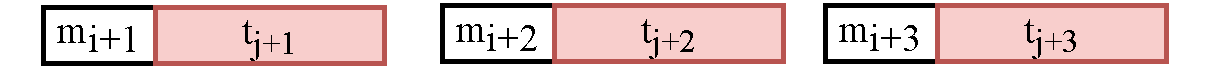
\includegraphics[width= \columnwidth]{img/MAC/TradMAC.pdf} 
    \caption{Traditional MAC}
        \vspace{.3cm}
    \label{fig:traditional}
    \end{subfigure}

    \begin{subfigure}{\columnwidth}
    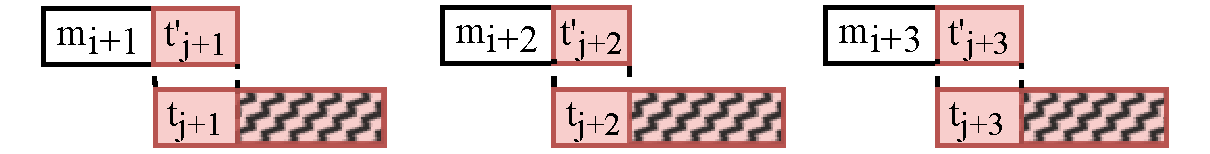
\includegraphics[width= \columnwidth]{img/MAC/TruncMAC.pdf}
    \caption{Truncate MAC}
    \label{fig:truncate}
    \end{subfigure}
    \caption{\small '$m_i$' represent the message and '$t_j$' represents the MAC (also called tag). Truncating the tag decreases the security~\cite{ProMAC1, badgeOfShame}.}
\end{figure}
The second direction is to use one tag across multiple messages using aggregate MAC or aggregate message techniques~\cite{aggregateMAC,compoundMAC, compundMAC_original}. Nonetheless, aggregating creates verification dependencies: the tag can only verify the integrity of the group if all of its dependent messages arrive correctly. In lossy or adversarial wireless settings (e.g., under jamming), losing even a single dependent message makes the tag unusable and enables denial-of-service against the integrity check~\cite{DoS_AggregateMAC,XOR_MAC,proMac2,when_And_How_Aggregate_In_Lossy_Channel}.

\begin{table*}[h]
	\centering
	\caption{Prior approaches vs.\ OptiMAC (qualitative comparison).}
	\label{tab:rw-compare}
	% \begin{tabular}{p{2.8cm}p{3.7cm}p{2.1cm}p{2cm}p{2.6cm}p{1.8cm}}
		\begin{tabular}{llllll}
			\toprule
			\textbf{Approach} & \textbf{Overhead handling} & \makecell[l]{\textbf{Jamming}\\ \textbf{resistance}} & \makecell[l]{\textbf{\# tag assigned} \\ \textbf{per~msg}} & \textbf{\# tag (n) vs. \# msg (m)} & \textbf{Tag size} \\
			\midrule
			Traditional MAC & None & Highest  & 1 (fixed) &$n=m$ (fixed) & High\\
			Short MAC~\cite{badgeOfShame} & Tag truncation & Highest &1 (fixed) & $n=m$ (fixed)& Low\\
			Agg. MAC~\cite{aggregateMAC,sequential_aggregate} & Grouping & Low &1 (fixed)&  $n\leq m$ (semi-flexible)& High\\
			Agg. msg~\cite{compundMAC_original,compoundMAC} & Grouping & Low &1 (fixed)&  $n\leq m$ (semi-flexible)& High\\
			ProMACs~\cite{ProMAC1, cuMAC} & \makecell[l]{Stateful multi-verification} & Low & $\geq 1$ (flexible)& $n=m$ (fixed) & Low\\
			SP-MAC~\cite{proMac2} & \makecell[l]{Golomb rulers based \\dependency assignment} & Medium & $\geq 1$ (flexible)& $n=m$ (fixed) & Low\\ 
			\textbf{OptiMAC} & \textbf{Optimizing dependencies} & \textbf{High} & \textbf{Optimized} &  $n\leq m$ \textbf{(fully flexible)} & \textbf{Optima} \\
			\bottomrule
		\end{tabular}
	\end{table*}


Armknecht et al.~\cite{ProMAC1} proposed the Progressive MAC (ProMAC) framework, which generalizes many aggregation schemes by maintaining an internal state (a buffer) that is updated with each new message and then used to generate tags. A notable realization of this framework, the Whips scheme, cross-assigns tags across multiple messages so that each message is verified several times. This allows shorter tags to achieve the same effective security level as a longer tag can provide in a traditional MAC~\cite{ProMAC1}. However, like aggregate MAC, Whips was designed for error-free channels. In practice, on jammed or lossy wireless links, Whip is susceptible to sandwich attack~\cite{proMac2}. In adversarial settings, an integrity-check scheme must therefore explicitly account for message loss and maximize goodput, which jointly accounts for the amount of message bits that is integrity verified and the total transmitted tag bits. Intuitively, goodput improves when tag overhead is reduced while ensuring that a equal or higher number of message bits remain verifiable. Directly optimizing this trade-off, however, is extremely challenging.

% : it requires simultaneously assigning tags to messages, evaluating the probability that each tag remains usable under loss and jamming, and selecting tag lengths that jointly influence both the numerator and denominator of the goodput expression. These interdependent decisions form a tightly coupled, combinatorial, and highly non-convex problem, rendering a single unified optimization approach exceedingly difficult.

To solve this problem, our proposed OptiMAC approach follows a divide-and-conquer strategy to improve the goodput by first maximizing the expected number of tag verification and second finding the optimal tag length. 

% Optimizing tag size according to the loss probability is important. Arbitrarily shortening tags could reduce the number of messages that satisfy security requirements and thus harm goodput; by first increasing the likelihood that each message is verified multiple times by different tags and only then truncating tag length within the security constraints, OptiMAC improves goodput without hindering the number of messages the receiver can verify.

% We evaluate OptiMAC on live UDP webcam streams over Wi-Fi and 5G, comparing against trad. MAC, aggregate MAC, and ProMAC baselines. Across a range of loss and jamming conditions, OptiMAC increases the realized verifications per message, therefore delivers higher or least similar goodput compared to existing methods. The gains come from aligning tag-to-message assignment with the channel condition first, and only then tuning tag length accordingly to the satisfy the security requirement.

\subsection*{Summery of contributions}

\textbf{Flexible integrity-check framework.} We propose OptiMAC, an extension of the Progressive MAC (ProMAC) framework, to enable applications to choose flexible arbitrary tag-to-message ratios and fine-tune the balance between integrity overhead and security.

\textbf{Optimization-based tag assignment.} We designed a novel optimization model that systematically assigns tags to messages so as to maximize the expected number of usable tags under packet loss and jamming. 

\textbf{Precomputed methods for online adaptation.}
OptiMAC enables applications to precompute optimal configurations for a range of channel conditions and then adapt to the appropriate configuration during online operation.


\textbf{Comprehensive evaluation.} Through large-scale simulations and real-world live UDP webcam streams over Wi-Fi and 5G, we evaluated OptiMAC Across a range of loss and jamming conditions. We demonstrate that OptiMAC achieves superior goodput while maintaining a $256$-bit security level, in particular, under periodic jamming.




Overall, OptiMAC unifies security, efficiency, resilience, and flexibility in a single framework, offering a practical and theoretically sound solution to integrity verification in lossy and adversarial communication environments.








\section{Preliminaries}\label{prelim}
To establish the foundation of our proposed framework, we begin by defining the essential performance metrics, including the Security Level Requirements and Goodput.

% \subsection*{Message Authentication Codes (MACs)}
% A Message Authentication Code (MAC), also referred to as tag, is a cryptographic tool that ensures the integrity and authenticity of a message. Formally, a MAC scheme is defined by \textbf{Tag Generation (Sig)}, which uses the key \( k \) and a message \( m \) to generate a MAC tag \( t \), thus \( t = \text{Sig}(k, m) \). Lastly, \textbf{verification (Vrfy)} which confirms the validity of the tag. Given a key \( k \), message \( m \), and received tag \( t \), the algorithm \( \text{Vrfy}(k, m, t) \) outputs either true (if the tag is valid) or false otherwise. MACs security level dependent exponentially on the length of the tag and additionally to the the strength of the underlying key and cryptographic algorithm.

\subsection*{Security Level Requirement}\label{sec_lvl_req}
Many applications specify a required security level $S$ (e.g., $S=256$ bits) per message. If each usable tag verification contributes $|t|$ bits of tag strength, then a message meets the security level requirement when it accumulates enough verifications so that the cumulative strength reaches $S$.
\subsection{Goodput Metric}
We use \emph{goodput} to quantify efficiency: the ratio of messages that are verified (received and met security level requirements) relative to the total bits transmitted (messages plus tags). 
\begin{equation}
    G = \dfrac{\sum\text{verified message bits}}{\sum\text{transmitted messages bits} + \sum\text{transmitted tag bits}}.
\end{equation}



\section{Literature Review}\label{literature_review}


Various integrity verification methods have been developed to reduce communication and computational overhead. The overhead imposed by Message Authentication Codes (MACs) is a significant issue in bandwidth-limited networks such as CAN~\cite{compoundMAC} and in high data rate applications within 5G networks~\cite{etsi_ts_133501_v17_5_0}. Truncated MACs have been proposed as a practical solution to mitigate this overhead. However, truncation comes at the expense of security strength, making the system more vulnerable to collision attacks~\cite{ProMAC1}.

Other overhead-reducing schemes, such as aggregate and compound MACs, minimize computational and communication overhead by verifying multiple messages with a single tag. While this approach eliminates the need to compute and transmit a MAC for every individual message, it introduces a critical weakness: the loss or corruption of any single packet within the group prevents the integrity verification of the entire set. This weakness arises because all messages contribute to the generation of the common MAC, making them mutually dependent. Consequently, the integrity check fails if even one message is missing, leaving the common MAC unusable.

To address this weakness, it is important to recognize that aggregate and compound MAC schemes were originally designed for error-free communication links, which makes them particularly susceptible to packet losses. Such losses may arise naturally in lossy channels or be deliberately introduced through jamming attacks, indicating the presence of an adversary~\cite{jamming_Servey, XOR_MAC, proMac2, DoS_AggregateMAC}. Detecting and preventing jamming is especially challenging in wireless environments. Random jamming, for example, mimics the behavior of a naturally lossy channel, making reliable detection extremely difficult~\cite{jamming_Servey}. Therefore, MAC overhead-reducing schemes must explicitly consider the impact of various jamming strategies, including random and periodic jamming, to ensure resilience under adversarial conditions.
% For example, if aggregate or compound MACs are implemented, an attacker can execute denial-of-service (DoS) attacks by jamming every $'n'$ packets. This is a much lower rate compared to that of traditional MACs~\cite{DoS_AggregateMAC, XOR_MAC}. Since the modification of a single packet in aggregated MAC schemes can prevent the verification of multiple messages due to their interdependencies, the attacker can significantly disrupt communication with minimal effort.
In this context, assessing the message-to-tag dependencies becomes essential to maintain the integrity and availability of the system in the presence of a jammer. Understanding these dependencies is vital for designing robust integrity verification schemes that can withstand packet losses and malicious attacks.


\subsection{Problem Background}
The earliest integrity-check overhead reduction approach can be traced to \cite{XOR_MAC_original}, which introduced an XOR-based aggregation technique that combines multiple digital signatures into a single compact signature. This method not only reduces the total size of transmitted signatures but also provides provable security guarantees\cite{boneh2003aggregate, XOR_MAC_original, XOR_MAC}. Building on this idea, \cite{aggregateMAC}~has applied the aggregation technique to MAC schemes, combining multiple tags into a single tag to reduce communication overhead. An alternative direction, explored in~\cite{sequential_aggregate, sequential_aggregate2, application_sequential_aggregation}, proposed sequential aggregation, where each new signature is computed over the current message concatenated with the preceding signature, effectively chaining multiple signatures into one. 
\begin{figure}[h]
    \centering
    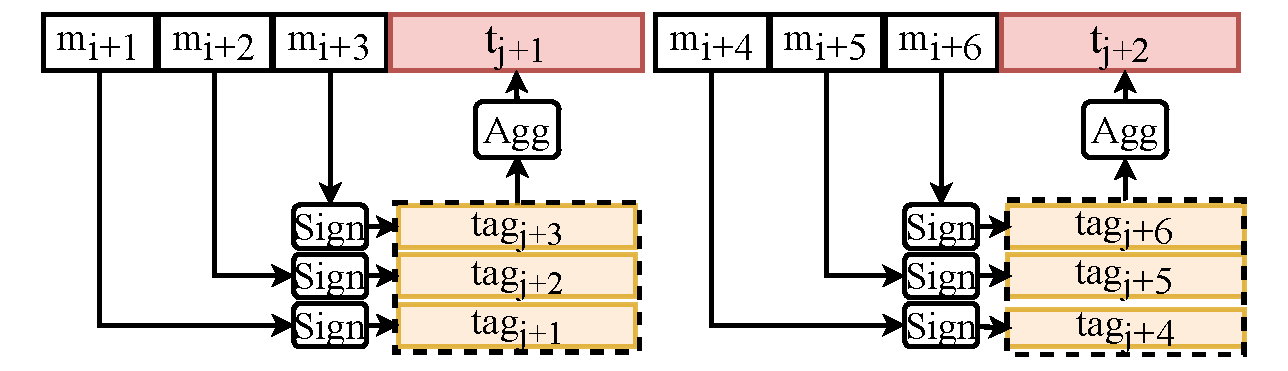
\includegraphics[width= \columnwidth]{img/MAC/AggMAC.pdf}
    \caption{Aggregate MAC~\cite{aggregateMAC}}
    \label{fig:AggMAC}
\end{figure}

Figure~\ref{fig:AggMAC} illustrates the MAC aggregation technique proposed in~\cite{aggregateMAC}. Alternative approach, as shown in Figure~\ref{fig:AggMAC}, involves aggregating messages to generate a single tag, transmitting the resulting tag for all aggregated messages~\cite{compoundMAC, stateful, compundMAC_original, miniMAC}. 
\begin{figure}[h]
     \centering
     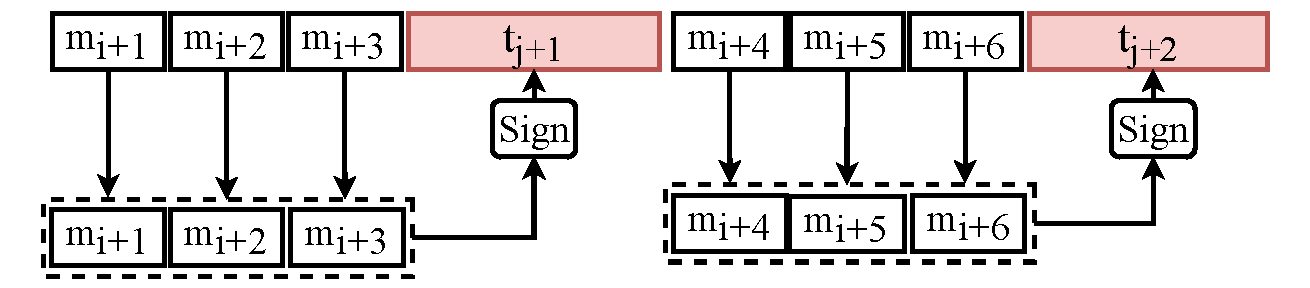
\includegraphics[width = \columnwidth]{img/MAC/CompMAC.pdf}
     \caption{Aggregate Messages~\cite{compundMAC_original}}
     \label{fig:compoundMAC}
\end{figure}
The 'Sign' operation indicates the MAC generation process, and 'Agg' depicts the aggregation step. While these two schemes are different in nature, from the message and MAC interdependency point of view, they behave the same. Thus, from now on, the aggregate MAC and aggregate message terminology might be used interchangeably.
 

 
% Our analysis focuses on the dependencies created during the aggregation step. Both aggregation approaches introduce similar vulnerabilities to packet losses. These dependencies can be exploited in jamming scenarios, leading to a significant risk of denial-of-service and reduced quality of service.

% \subsection{Related work}

In~\cite{ProMAC1}, the Progressive MACs framework is introduced, which provides a novel approach to generalize all the previous MAC aggregation schemes. Progressive MACs framework utilizes an internal state mechanism that is updated with every new message and a tag generation mechanism that inputs from the internal state. Figure~\ref{fig:proMAC} illustrates one possible realization of a progressive MAC framework, called Whips, with an internal state of size three.
\begin{figure}[h]
    \centering
    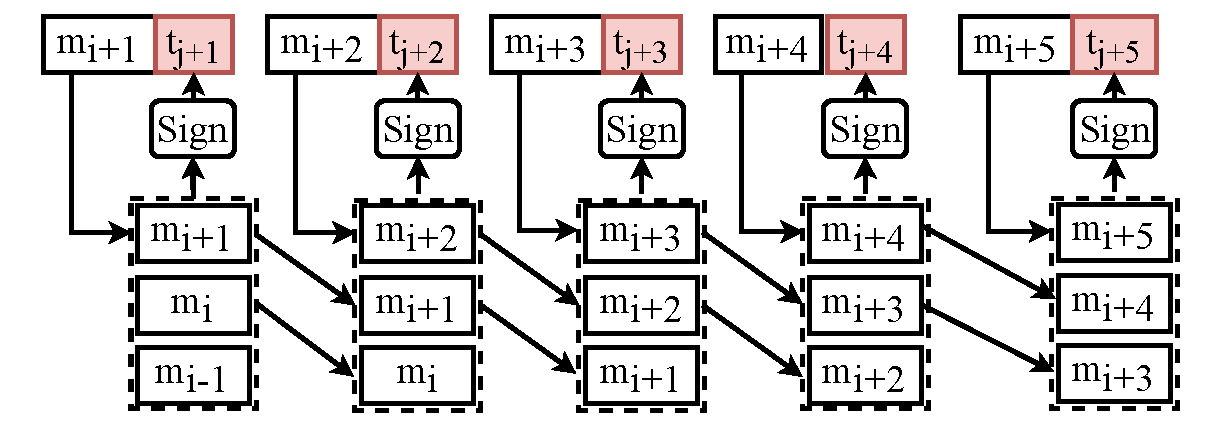
\includegraphics[width = \columnwidth]{img/MAC/ProMAC.pdf}
    \caption{ProMACs~\cite{ProMAC1, cuMAC} cross-assigns message to tag. This Figure is reproduced from~\cite{proMac2}.}
    \label{fig:proMAC}
\end{figure}
As shown in Figure~\ref{fig:proMAC}, the message $m_{i+1}$ is involved in the generation of tags $t_{j+1}$, $t_{j+2}$, and $t_{j+3}$. This way, the message $m_{i+1}$ will be verified by the three tags, which means to successfully modify $m_{i+1}$, an attacker would need to guess all three tags correctly, equivalent in security to using a tag three times as large. For instance, if a message requires the security level of a 256-bit tag, a Progressive MAC with a state of size three could achieve this with 86-bit tags, as each message is verified three times. This state mechanism allows Whips to gradually verify the integrity of packets as more tags are received, effectively increasing the security level over time without requiring full-length tags for each packet~\cite{ProMAC1}.

Therefore, Progressive MAC-based schemes~\cite{ProMAC1, proMac2, cuMAC, miniMAC} are not confined to fixed-length tag configurations. Depending on security requirements and bandwidth constraints, they can employ truncated tags that, through cumulative verification across multiple packets, offer security guarantees comparable to traditional MACs~\cite{ProMAC1}. By tuning parameters such as tag length, state-update rules, and internal state size, the Progressive MAC framework can adjust to application constraints~\cite{ProMAC1}. However, despite this versatility, the ProMAC framework lacks a systematic method for determining optimal parameter choices for different application constraints. Without a systematic approach, designing a good-performing system becomes extremely difficult. This is even more critical in adversarial environments, where periodic or random packet loss can severely attack the integrity check scheme.
 
To address this limitation, we propose OptiMAC, a graph-based mapping approach that enables a systematic design and analysis of the ProMAC framework. This graph-based method systematically analyzes and adjusts dependencies between messages and tags, resulting in an optimized structure that maximizes the number of verifiable packets under conditions of high packet loss, achieving optimal security tailored to specific channel conditions.



\subsection{Limitations in Adversarial Environments}
% The proposed methods are promising solutions for MAC overhead reduction but are not designed for lossy channels.
% In~\cite{when_And_How_Aggregate_In_Lossy_Channel}, they have studied the effect of the packet loss on the mentioned schemes where they concluded that channel condition has a remarkable influence on performance. For instance, in the Aggregate MAC, as can be seen from Figure~\ref{fig:AggMAC}, if any of the messages in the group of $\{m_{i+1}, m_{i+2}, m_{i+3}\}$ is lost or modified, the other messages will not be verified and may be discarded.
The limitations of MAC or message aggregation schemes in adversarial scenarios have been previously pointed out. Kolesnikov et al.~\cite{DoS_AggregateMAC} demonstrated that MAC overhead-reducing schemes can increase the system's vulnerability to DoS attacks. To address this, Kolesnikov et al. proposed a "shifted bitwise XOR" approach to mitigate the impact of packet loss on the verification of other messages~\cite{DoS_AggregateMAC}.

Wagner et al.~\cite{proMac2}, introduce SP-MAC, a resilience-oriented authentication scheme extending the Progressive MAC (ProMAC) framework with a combinatorial construction based on Golomb rulers and generalized $g$-Sidon sets~\cite{proMac2}. This dependency structure is designed to limit the effect of a message loss on the other messages, making it more resilient in adversarial scenarios. Despite the SP-MAC claim of having the \emph{optimal} dependency distribution, it lacks quantifiable objectives. The provable guarantees are controllable latency and controllable effect of message-loss on other messages. Though this doesn't by it self guarentee optimal latency or optimal goodput of the overall system. Moreover, Similar to many other schemes, the number of tags that are required to be genereted equals to the number of messages, whereas aggregate MAC and Our proposed OptiMAC allow flexibility on the number of tag used per message, reducing computational overhead. 

It is evident from~\cite{proMac2, DoS_AggregateMAC, when_And_How_Aggregate_In_Lossy_Channel} that grouping messages or aggregating tags to reduce overhead introduces verification dependencies between messages. These dependencies can add latency and make the system vulnerable to jamming. While some prior work~\cite{DoS_AggregateMAC, proMac2} has recognized this problem and proposed heuristic solutions, our study presents an optimization approach to find the optimal parameters in adversarial environments.

In summary, progressive MAC introduces a framework that generalizes all MAC aggregation schemes through an evolving internal state and an arbitrary update and tag generation function. However, the lack of guidance to find the optimum settings for this framework, especially in challenging under-attack environments, leaves a gap that we are addressing in this paper. Our proposed OptiMAC framework maps the state and the update functions of the ProMAC framework to a graph, providing a systematic approach to analyze and optimize any MAC aggregation schemes. Addressing this issue is critical for improving the efficiency and security of communication systems, particularly in adversarial wireless environments. 


%Based on this mapping we develop an optimization model enables to also application of different MAC schemes under varying conditions, offering robust guidance for designing more resilient wireless communication systems.


% A critical research gap exists in finding the optimal dependency distribution between tags and messages to maximize verified throughput and minimize latency in lossy channels. This paper addresses this issue by systematically studying the dependency problem, aiming to optimize the verification process for different channel conditions.
% The current methods, while effective in reducing overhead, often introduce dependencies that can lead to increased latency and vulnerability to attacks, especially in environments with high packet loss rate. 












\section{Threat Model}\label{Threat Model}
In this work, we consider an adversarial setting modeled by a simplified version of the Dolev-Yao attacker model~\cite{Dolev-Yao}. The attacker has the capability to inject, drop, or modify packets transmitted over the network. Specifically, the attacker can introduce forged packets into the communication channel with the intent of deceiving the receiver or disrupting the communication protocol. The attacker can also intercept and remove packets from the communication channel, preventing their delivery to the intended recipient. Additionally, the attacker can alter the content of transmitted packets, potentially corrupting the data or causing the receiver to accept false information.

We assume that the attacker does not possess the cryptographic keys used for securing the communication. Consequently, the attacker cannot decrypt encrypted messages or generate valid encrypted messages and authentication tags. The inability to decrypt or correctly encrypt messages limits the attacker to manipulate the transmission medium and observable packet structures without understanding or creating valid encrypted content.

This threat model focuses on preserving the integrity and authenticity of messages in the presence of an active adversary capable of tampering with the communication channel but lacking the cryptographic keys necessary to compromise confidentiality or generate valid cryptographic tokens. 

\section{Design Goals}\label{Design Goals}
The security of integrity checks is fundamentally dependent on the length of the MAC employed; this is also referred to as the security level in~\cite{ProMAC1}. In the conventional approach, enhancing security involves utilizing larger tags, which incurs additional overhead. Instead of merely increasing the length or number of tags, we focus on optimizing tag-to-message dependencies to effectively enhance performance and security without increasing the actual tag length or the total number of tags. The followings will summarize our design goals.

\noindent\textbf{G1: High Goodput.}  A high-goodput system maximizes the message bits that have been verified above the required security threshold while at the same time minimizing the total tag bits transmitted.

\noindent\textbf{G2: Meeting Security Level Requirements.} Increasing the number of tag bits per message results in an exponential enhancement of integrity check security~\cite{ProMAC1}. Increasing the tag length above some threshold would be unnecessary for practical application and would have a reverse effect on the goodput performance. Thus, the tag length must be optimized in a way that maximizes the goodput while maintaining the security requirements. 
% While the Whips algorithm leverages this concept and reduces the tag size~\cite{ProMAC1}, it does it in a heuristic manner and does not necessarily meet the security level requirement in adversarial scenarios. In contrast, an ideal approach would determine the optimal tag length balancing security and goodput.


\noindent\textbf{G3: Systematic, Adversary-Aware Optimization.}
A desirable MAC scheme should offer a principled, model-driven procedure, rather than heuristic tuning, for operation under lossy and adversarial conditions. Given fixed operating parameters (number of messages, number of tags, and a loss/jamming probability), it should systematically compute the optimum message-to-tag assignment, and thereafter finds the optimum tag length to maximizes the goodput of the system.


\noindent\textbf{G4: Flexible Tag-to-Message Ratio.} 
The system should support arbitrary effective average tags per message (e.g., $2/3$), rather than only the reciprocal ratios ($1/g$) imposed by rigid grouping of the Aggregate MAC.


% While MILP is known to be NP-hard and may require significant computation time, we address this challenge by precomputing solutions for various parameter configurations. As soon as an environment change is detected, the system can immediately switch to the corresponding precomputed solution.

 % To achieve this, we introduce a novel mapping of tag-to-message assignments to a graph denoted as the dependency graph. The utilization of the dependency graph facilitates the analysis and optimization of the dependencies between messages and their assigned tags. Our systematic approach guarantees optimal security under varying channel conditions for any given number of messages and tags.

% Since the framework that is presented in this paper assumes the number of messages, tags, and attack rate as fixed parameters for the mathematical model. Then, the framework will be able to provide the optimal dependency graph for the given inputs.

% Given the parameters, the framework solves an MILP problem. MILP problems are known as NP-Hard problems, which can take a long time to solve. One might argue that MILPs are too slow to be used for rapid time-varying parameters. However, we point out that the computation can be done beforehand for different scenarios of parameters. Then the appropriate optimal assignment can be deployed as soon as the environment change is detected. With this scheme, the presented works can be implemented in real-world applications.




\section{Dependency Mapping}\label{Novel Mapping}

Grouping messages or aggregating tags introduces dependencies in the verification process, making the system more vulnerable to jamming attacks. By constructing the dependency graph, we model the relationships between messages and tags.

% Next, we define critical metrics: Comparative Efficiency ($CE$), authentication ($\textbf{A}$), latency ($\textbf{L}$), strength number, number of tag-bits per message,\tianwei{should we also have abbreviation for these two metrics here?} and goodput ($G$). These metrics are essential for assessing the robustness and resiliency of MAC overhead-reducing schemes under jamming or insider attacks.\tianwei{some metrics in Table 1 are not mentioned here, does that mean they are not critical? should we add some explanations for why we consider these are essential?}

% \begin{table}[h]
% \centering
% \caption{Summary of Metrics and Acronyms}
% \begin{tabular}{|c|c|}
% \hline


% \multicolumn{2}{|c|}{ \cellcolor[HTML]{D3D3D3} \large \textbf{Vectors} }\\ \hline

% \textbf{Metric} & \textbf{abbrv.} \\ \hline

% Authentication & \textbf{A} \\\hline
% Expected Number of Authentications & $E[\textbf{A}]$ \\ 
% \hline 
% Authenticationd Latency & \textbf{L} \\ \hline

% Tag Usability & \textbf{U} \\ \hline

% Dependency  Matrix & \textbf{X} \\ \hline
% % \multicolumn{2}{c}{}\\
% \hline
% \multicolumn{2}{|c|}{\cellcolor[HTML]{D3D3D3} \large Scalars}\\ \hline
% \textbf{Metric} & \textbf{abbrv.} \\ \hline

% Comparative  Efficiency &$CE$  \\ \hline


% Goodput & $G$ \\ \hline

% Integrity Security & $IS$ \\ \hline

% Strength Number &$SN$\\ \hline
% \end{tabular}
% \label{tab:metrics}
% \end{table}



\subsection*{\textbf{Dependency Graph}}
Assuming the general case of a system with '$m$' messages and '$n$' tags where:
\begin{align}
    \textbf{m} = \{m_1, m_2, \cdots, m_i, \cdots, m_m\}\nonumber\\
    \textbf{t} = \{t_1, t_2,\cdots, t_j,\cdots, t_n\}\nonumber
\end{align}

We define the dependency graph such that \( DG = (\textbf{V}, \textbf{E}) \) is an undirected graph representing the tag-to-message dependencies.  \( DG \) is defined as follows:
\begin{equation}
    \textbf{V}_1 = \{m_i\mid i \in \{1,\cdots,m\}\},\nonumber
\end{equation}
is the set of vertices, where each \( m_i \) represents a message.
\begin{equation}
    \textbf{V}_2 = \{t_j\mid j \in \{1,\cdots,n\}\}, \nonumber
\end{equation}
is the set of vertices, where each \( t_j \) represents a tag, And 
\begin{equation}
    \textbf{V} = \textbf{V}_1 \cup \textbf{V}_2\nonumber.
\end{equation}
\begin{equation}
    \textbf{E} \subseteq\{ (u, v) \mid u \in \textbf{V}_1, v \in \textbf{V}_2\}, \nonumber 
\end{equation}
is the set of undirected edges, where an edge \( \{m_i, t_j\} \in \textbf{E} \) signifies that tag \( t_j \) verifies message \( m_i \).

Each vertex \( v \in \textbf{V} \) can be a message or tag, and each edge \( e \in \textbf{E} \) indicates a tag-to-message assignment. Figure~\ref{fig:proMAC_graph} visualizes the dependency graph for the progressive MAC.
\begin{figure}[!h]
    \centering
    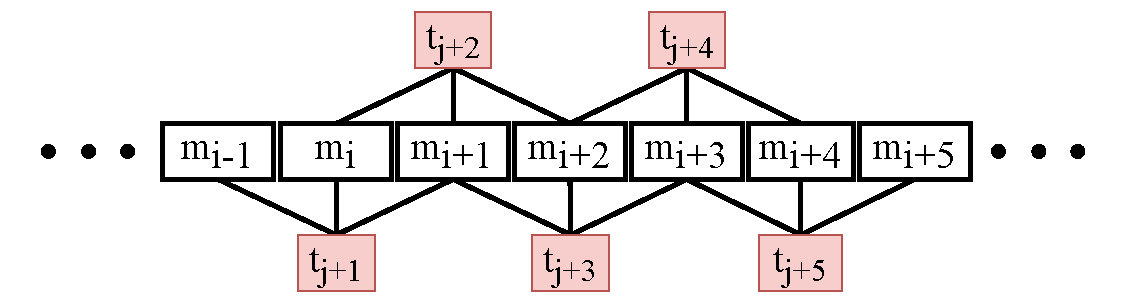
\includegraphics[width = .9\columnwidth]{img/graph/Whip_Graph.pdf}
    \caption{Whips dependency graph with internal state size of 3.}
    \label{fig:proMAC_graph}
\end{figure}

\subsection*{\textbf{Dependency Matrix (X)}}Based on the dependency graph, we define the dependency matrix \( X \), where the rows correspond to messages and the columns correspond to tags. The entries of the matrix are defined as follows:
\begin{equation}
X_{i,j} = 
\begin{cases} 
1 & \text{if message } m_i \text{ is assigned to tag } t_j \\
0 & \text{otherwise}
\end{cases}
\end{equation}

For example, the dependency matrix of the Whips scheme, as shown in Figure~\ref{fig:proMAC_graph}, is as follows:
\setlength{\tabcolsep}{1.9pt}
\renewcommand{\arraystretch}{1.3}
\[
\begin{array}{ccccccccc}
\multirow{12}{*}{\textbf{X} =}& & \textcolor{red!40}{t_1} & \cdots & \textcolor{red!40}{t_{j+1}} & \textcolor{red!40}{t_{j+2}} & \textcolor{red!40}{t_{j+3}}  &  \cdots & \textcolor{red!40}{t_n} \\
\cline{3-3}
\cline{9-9}
&\textcolor{blue!60}{m_1}     & \multicolumn{1}{|c}{1} & \cdots  & 0 & 0 & 0 & \cdots & \multicolumn{1}{c|}{0} \\
&\vdots & \multicolumn{1}{|c}{\vdots} & \ddots & \vdots & \vdots & \vdots & \ddots &  \multicolumn{1}{c|}{\vdots} \\
&\textcolor{blue!60}{m_{i-1}} & \multicolumn{1}{|c}{0} &  \cdots & 1 & 0 & 0 & \cdots & \multicolumn{1}{c|}{0} \\
&\textcolor{blue!60}{m_{i}}   & \multicolumn{1}{|c}{0} &  \cdots & 1 & 1 & 0 & \cdots & \multicolumn{1}{c|}{0} \\
&\textcolor{blue!60}{m_{i+1}} & \multicolumn{1}{|c}{0} &  \cdots & 1 & 1 & 1 & \cdots & \multicolumn{1}{c|}{0} \\
&\textcolor{blue!60}{m_{i+2}} & \multicolumn{1}{|c}{0} &  \cdots & 0 & 1 & 1 & \cdots & \multicolumn{1}{c|}{0} \\
&\textcolor{blue!60}{m_{i+3}} & \multicolumn{1}{|c}{0} &  \cdots & 0 & 0 & 1 & \cdots & \multicolumn{1}{c|}{0} \\
&\vdots & \multicolumn{1}{|c}{\vdots} & \ddots & \vdots & \vdots & \vdots  & \ddots &  \multicolumn{1}{c|}{\vdots} \\
& \textcolor{blue!60}{m_m} & \multicolumn{1}{|c}{0} & \cdots & 0 & 0 & 0 &    \cdots & \multicolumn{1}{c|}{1} \\
\cline{3-3}
\cline{9-9}
\end{array}
\]


% \[
% \begin{array}{ccccccc}
% \multirow{8}{*}{X =}& & \textcolor{red!40}{r_{j+1}} & \textcolor{red!40}{r_{j+2}} & \textcolor{red!40}{c_{j+1}} & \textcolor{red!40}{c_{j+2}}  &  \textcolor{red!40}{c_{j+3}} \\
% \cline{3-3}
% \cline{7-7}
% &\textcolor{blue!60}{m_{i+1}} & \multicolumn{1}{|c}{1} & 0 & 1 & 0 &\multicolumn{1}{c|}{0} \\
% &\textcolor{blue!60}{m_{i+2}} & \multicolumn{1}{|c}{1} & 0 & 0 & 1 &\multicolumn{1}{c|}{0} \\
% &\textcolor{blue!60}{m_{i+3}} & \multicolumn{1}{|c}{1} & 0 & 0 & 0 &\multicolumn{1}{c|}{1} \\
% &\textcolor{blue!60}{m_{i+4}} & \multicolumn{1}{|c}{0} & 1 & 1 & 0 &\multicolumn{1}{c|}{0} \\
% &\textcolor{blue!60}{m_{i+5}} & \multicolumn{1}{|c}{0} & 1 & 0 & 1 &\multicolumn{1}{c|}{0} \\
% &\textcolor{blue!60}{m_{i+6}} & \multicolumn{1}{|c}{0} & 1 & 0 & 0 &\multicolumn{1}{c|}{1} \\

% \cline{3-3}
% \cline{7-7}
% \end{array}
% \]

\subsection*{\textbf{Status Vector}} Let \( \mathbf{M} \) and \( \mathbf{T} \) denotes the status vector, where each entry indicates if the message or tag is correctly received or lost (modified or jammed). \( \mathbf{M} \) is defined as follows:
\[
\mathbf{M} = 
\begin{bmatrix}
M_1 & M_2 & M_3 & \cdots& M_i & \cdots & M_m 
\end{bmatrix}
\]
Where \( M_i = 1 \) if message \( m_i \) is successfully received, and \( M_i = 0 \) otherwise. The tag status vector \( \mathbf{T} \) is defined as follows:
\[
\mathbf{T} = 
\begin{bmatrix}
T_1 & T_2 & T_3 & \cdots & T_j & \cdots & T_n
\end{bmatrix}
\]
Where \( T_j = 1 \) if tag \( t_j \) is successfully received, and \( T_j = 0 \) otherwise. 


% Assuming that tags and messages are sent separately is the most general case, covering all possible implementations. By simply setting the tag status vector to all 1s, we can represent implementations where tags are sent alongside the messages. This is based on the assumption that the tag $t_j$ next to message $m_i$ must at least verify $m_i$. 
% If the packet containing both $m_i$ and $t_j$ is lost, even though in the tag status vector $T_j =1$, the inherent relationship between $m_i$ and $t_j$ means that $M_i = 0$ should effectively result in $T_j = 0$.






\subsection*{\textbf{Tag Usability (U)}}
A tag is usable if the tag and all the dependent messages are correctly received. Let $U_j = 1$ if tag $t_j$ is usable, and $U_j = 0$ otherwise. A usable tag can authenticate all the messages that are dependent on it, whereas an unusable tag can not verify any messages. the $U_j$ in the tag usability vector \( \textbf{U} =  \{U_1, ..., U_n\}\) is given by:
\begin{equation}    
U_j = T_j \cdot \prod_{i \in \{i \mid X_{ij} = 1\}} M_i
\end{equation}

\subsection*{\textbf{Authentication (A)}}
Let $A_i$ denote the number of usable tags verifying message $m_i$. The $A_i$ from the authentication vector $\textbf{A} = \{A_1, ..., A_m\}$ is as follows:
\begin{equation}
    A_i =  \sum_{j \in \{j \mid X_{ij} = 1\}} U_j 
\end{equation}
For example, for the the Whips in Fig.~\ref{fig:proMAC}, if all tags and messages are correctly received, vector \( A \) from \( i-1 \) to \( i+5 \) will be as follows:
\begin{equation}
    \textbf{A} = [\cdots, 3, 3, 3, 3, 3, 3, 3, \cdots]
\end{equation} 
However, in the case that message \( m_{i+2} \) is lost, tags \( t_{j+2} \), \( t_{j+3} \), and \( t_{j+4} \) become unusable. Therefore, vector \( A \) will be as follows:
\begin{equation}\label{proMAC_packetLoss_example}
    \textbf{A} = [\cdots, 3, 2, 1, 0, 1, 2, 3, \cdots]
\end{equation}

To calculate the expected authentication vector, the binary status of messages and tags is substituted with the probability that they are successfully received. Let \( P_i \) be the probability that message \( m_i \) is successfully received, and let \( Q_j \) be the probability that tag \( t_j \) is successfully received. The probability that tag \( U_j \) is usable is as follows:
\begin{equation}
    Pr(U_j = 1) = Q_j \cdot \prod_{i \in \{i \mid X_{ij} = 1\}} P_i,
\end{equation}
then the expected number of usable tags for a given message $m_i$ can be expressed as:
\begin{equation}\label{E[A]}
E[A_{i}] = \sum_{j \in \{j \mid X_{ij} = 1\}} U_j \cdot Pr(U_j=1)
\end{equation}
Where \( U_j=1 \) represents a usable tag and \( U_j=0 \) otherwise.
% \subsection{Authentication Probability}
% Since message $m_i$ can be verified if there is at least one usable tag that verifies $m_i$, the authentication probability for message $m_i$ is given by:
% \begin{align}
% Pr(A_i > 0) & = 1-Pr\text{(no tag verifies message } m_i) \nonumber \\
%      & = 1- \prod_{j \in \{j \mid X_{ij} = 1\}} \left(1- Pr(U_j = 1)\right)
% \end{align}
%For example, in the Whips shown in Fig.~\ref{fig:proMAC_graph}, if:
%$$P_i = p \quad \forall i \quad i \in \{1, \cdots, m\}, $$
%$$Q_j = q \quad \forall j \quad j \in \{1, \cdots, n\}, $$ 
%the expected number of usable tag for $m_i$ deriving from Equation~(\ref{E[A]}) is given by:
%\begin{equation}
%E[A_i]  = 3qp^3 
%\end{equation}

This probabilistic formulation allows for the evaluation of the authentication process under varying channel conditions, providing the necessary cornerstone for optimizing the tag-to-message assignments to enhance security, reliability, and performance.



\section{Optimization Model}\label{Proposed Scheme}
% Our proposed scheme, OptiMAC, extends the Progressive MAC (ProMAC) framework
% with an optimization layer that adapts the allocation of tags to both channel
% conditions and application requirements. Unlike prior approaches that employ a
% fixed tag-to-message ratio (TMR), OptiMAC allows any fractional assignment,
% thus flexibly trading off integrity assurance and communication overhead. The
% design is guided by four goals (G1–G4), and each part of the scheme is
% constructed to directly address these goals.

% OptiMAC maintains a running state that evolves with each new message and
% produces tags covering multiple overlapping subsets of messages. Instead of
% enforcing a one-tag-per-message rule, the scheme optimizes both the length of
% tags and their distribution across messages, ensuring that every message can
% be verified by several tags with controlled redundancy. This structure enables
% adaptability and robustness even under severe packet loss or adversarial
% jamming.

% With respect to G1 (Security), OptiMAC inherits the cryptographic foundation
% of ProMAC, where domain-separated pseudorandom functions (PRFs) are used to
% generate tags. Forging a valid set of tags requires producing multiple
% independent MACs, so the adversary’s success probability decreases
% exponentially with the number of required forgeries. By enforcing a 256-bit
% security budget across tags, the scheme provides strong protection against
% tampering while splitting this budget flexibly across shorter tags.

% For G2 (Efficiency), OptiMAC improves upon the rigid one-tag-per-message rule
% by enabling arbitrary tag-to-message ratios such as $2/3$ or $3/5$. This
% contrasts with aggregate MACs that are limited to discrete values of $1/n$.
% By distributing the same overall security budget across fewer or shorter tags,
% OptiMAC increases throughput while preserving verifiable integrity.

% In terms of G3 (Resilience to Loss and Jamming), the scheme leverages
% overlapping tag coverage. Each message is protected by multiple tags generated
% at different stages of the state evolution, so even if some tags are lost due to random or periodic jamming, other tags covering the same message still
% enable verification. This design avoids the all-or-nothing failure mode of
% aggregate MACs and maintains performance under highly adversarial conditions.

% Finally, G4 (Flexibility) is achieved through dynamic adaptation. OptiMAC can
% be tuned to prioritize higher throughput by reducing the TMR or greater
% robustness by increasing redundancy. Because the optimization considers
% measurable parameters such as message length, security requirement, and
% channel quality, the scheme can be configured in real time to match the needs
% of diverse applications ranging from low-latency communication to
% mission-critical secure links.

% In summary, OptiMAC unifies the goals of security, efficiency, resilience, and
% flexibility in a single framework. By discarding the traditional notion of
% “one message, one tag” and instead treating integrity as an optimizable
% resource, the scheme offers adaptability and performance advantages that prior
% approaches cannot provide.The detailed nomenclature for the mixed-integer linear program (MILP) model is provided in Table \ref{tab:nomenclature}.
Our proposed scheme, OptiMAC, extends the Progressive MAC (ProMAC) framework
with an optimization layer that determines how tags are generated, distributed,
and assigned to messages.

\begin{table} [htbp]
        
	\footnotesize
	\begin{center}
		\caption{\small Nomenclature for the OptiMAC's optimization model} \label{tab:nomenclature}
		\vspace{1ex} {
			\begin{tabular}{|l|l|}
				\hline
				\it{Sets} & {Description}\\ \hline
				$I$ &  Set of message indices $\{1,\ldots,m\}$ \\
				$J$ & Set of tags indices $\{1,\ldots,n \}$  \\
                    $K$ & Set of possible number of messages that can be  \\
                        & assigned to a tag $\{0,\ldots, m\}$  \\
				    % & \\
				\hline\it{Decision Variables} & {Description}\\ \hline
				$x_{ij}$  & Binary variables representing message assignments \\
         				   & to tag. Equal to 1 if message $i$ is assigned to tag $j$. \\
                              % &   \\
                    $z_{j}^k$ & Binary variables representing the total number of\\
                              & messages assigned to tag $j$. Equal to 1 if $k$ \\
                              &  messages are assigned to tag $j$.\\
                    $y_{ij}^k$ & Binary variables representing the combination of a \\
                               & message, its tag, and the total count of messages\\
                               & assigned to that tag. Equal to 1 if message $i$ is \\
                               & assigned to tag $j$, and there are $k$ messages \\ & assigned to that tag.\\
                    $U_{ij}^k$ & Expected value of tag $j$ being usable for message $i$ \\
                    &if message $i$ is assigned to tag $j$, and there are \\
                    & $k$ messages assigned to tag $j$.\\
                   $A^\prime$ & Dummy variable for equally representing the expected  \\
                    & number of usable tags across all the messages\\
                               % & \\
				\hline\it{Parameters} & {Description}\\ \hline
    
				$w^k (p,q) $ & Pre-calculated authentication probabilities with respect\\
                                     &  to $p, q$ for a tag with k number of assigned messages\\
				%$A^s$ & Uncertain crop yield under scenario $s$ (bu/acre)\\
				$p$ & Success probability of each message \\
                    $q$ & Success probability of each tag \\
				\hline
			\end{tabular}
		}
	\end{center}
\end{table}



% At its core, OptiMAC maintains a running state that evolves with each message,
% while tags are produced to cover multiple overlapping subsets of messages.
% Unlike traditional schemes that force a single tag per message, or aggregate
% MACs that can only support discrete ratios such as $1/n$, OptiMAC permits any
% fractional tag-to-message ratio. This flexibility ensures that every message is
% covered by at least one tag and often by several tags, so that verification
% remains possible even if some tags are lost. In practice, this allows OptiMAC
% to meet stringent security requirements while improving throughput and
% robustness under jamming.

% To achieve this flexibility systematically, we design an optimization module that determines how tags should be assigned to messages to maximize the expected number of expected usable tags. The objective function is to maximize the expected tag usability, as shown in equation~\eqref{eq:objective_sum}, where the contribution of each tag to each message is calculated in equation~\eqref{eq:message_auth_value}. Additional constraints ensure the consistency of assignments: equations~\eqref{eq:agg_count} and~\eqref{eq:single_agg} represent the total number of messages associated with each tag, equation~\eqref{eq:assign_y} defines message-to-tag assignment variables, equation~\eqref{eq:equivalent_A} balances the distribution of usable tags across messages, and equation~\eqref{eq:tag_every_message} guarantees that each message is covered by at least one tag. The remaining constraints enforce the binary nature of the decision variables. The complete mathematical formulation is presented in the Appendix for clarity and reproducibility.

% A key challenge arises because the expected usability function
% (Equation~\eqref{E[A]}) is nonlinear. To address this, we introduce an
% auxiliary variable $k$ representing the number of messages assigned to each
% tag. Let \(w^k_{ij}\) denote pre-computed authentication probabilities for
% message–tag assignments, and let \(U^k_{ij}\) represent the probability that
% tag $t_j$ is usable for message $m_i$ given $k$ assignments. By introducing
% binary variables \(y^k_{ij}\) to select the appropriate $w^k_{ij}$, we
% linearize the model into a mixed-integer linear program (MILP). Although this
% increases complexity, it allows us to leverage efficient solvers such as Gurobi
% to obtain optimal assignments under realistic settings. The implementation is
% developed in Python 3.9.6 and uses Gurobi version 11.0.2 as the solver. For
% transparency, our optimization codebase is available in a GitHub repository,
% with the link removed here to preserve anonymity in the review process.


Maximizing the $E[A]$ ensures  goals G1 and G2. Therefore, we have modeled this problem as follows:
\begin{align}
\text{max \hspace{.2cm}} & \sum\limits_{i \in I}\sum\limits_{j \in J}\sum\limits_{k \in K}  U_{ij}^k \label{eq:objective_sum} \\
% \text{min\hspace{.2cm}}  & |t_j| \\
\text{\hspace{.3cm}} s.t.  & \nonumber \\
% &\sum\limits_{i \in I}\sum\limits_{j \in J}\sum\limits_{k \in K}  U_{ij}^k > \tau& \label{eq:objective_sum} \\
& w^k y_{ij}^k |t_j|=  U_{ij}^k & \forall i \in I, j \in J, k \in K \label{eq:message_auth_value}\\
& \sum\limits_{i \in I} x_{ij} = \sum\limits_{k \in K} k z_{j}^k & \forall j \in J \label{eq:agg_count}\\
& \sum\limits_{k \in K} z_{j}^k \leq 1 & \forall k \in K \label{eq:single_agg}\\
& x_{ij} + z_{j}^k \geq 2 y_{ij}^k & \forall i \in I, j \in J, k \in K \label{eq:assign_y}\\
& \sum\limits_{j \in J} \sum\limits_{k \in K} U_{ij}^k = A^\prime & \forall i \in I \label{eq:equivalent_A}\\
& \sum\limits_{j \in J} x_{ij} \geq 1 & \forall i \in I \label{eq:tag_every_message}\\
& A^\prime \geq 0 \\
& x_{ij}, z_{j}^k, y_{ij}^k \in \{0,1\}  
\end{align}
The objective function is to maximize the expected number of usable tags for all messages \eqref{eq:objective_sum}. The expected tag usability of each message for its respective tag when in total $k$ messages are assigned to that tag is calculated in equation \eqref{eq:message_auth_value}. Equations \eqref{eq:agg_count} and \eqref{eq:single_agg} ensure the total number of messages assigned to each tag is represented accurately, while equation \eqref{eq:assign_y} handles the assignments for each message, tag, and assignment combinations. During our test runs, we noticed that the expected number of usable tags is not equally distributed. To ensure the equal distribution, equation ~\eqref{eq:equivalent_A} is incorporated. Finally, equation \eqref{eq:tag_every_message} makes sure each message is assigned to at least one tag. The remaining constraints are the binary restrictions on the decision variables.

% We have designed an optimization technique, an important block of optiMAC, that is capable of achieving optimum security. By employing mathematical programming, we developed a systematic approach to ensure the scheme achieves optimal expected security for each combination of tag and message numbers under varying loss rates, addressing goal G3. In designing a MAC scheme, security requirements—such as the number of bits that must verify each message—are typically predefined and fixed. As a result, the parameters available for optimization include the number of tags, the size of the tags, and the assignment of tags to messages. By strategically assigning messages to tags to maximize $E[\textbf{A}]$, we ensure optimal security is maximized, fulfilling goal G2. Moreover, by increasing the number of tags in every step we can find the optimum goodput to satisfy the design goal G1. Therefore, we formulate the optimization problem as follows:

 % why b is not in the objective 

% why k is there 
Equation \eqref{E[A]} is highly non-linear and requires linearization to be used in MILP formulation. Let \( w^k_{ij} \) be the pre-calculated authentication probability values for all possible message-to-tag assignments, where the superscript \( k \) represents the number of messages assigned to tag \( j \). 

Note that since the usability vector is a binary random variable where \( U_j \in \{0,1\} \), the probabilities and expected values are equivalent and these terms can be used interchangeably for clarity. Let \( U^k_{ij} \) represent the probability that tag \( t_j \) is usable for message \( m_i \) when a total of \( k \) messages are assigned to tag \( t_j \). By maximizing the summation of \( U^k_{ij} \) over \( j, i, k \), we maximize the expected number of usable tags for all messages.

In this model, \( y^k_{ij} \) will be set to one to assign the correct pre-calculated \( w^k_{ij} \) to \( U^k_{ij} \). While the introduction of the variable \( k \) linearizes the model, it increases computational complexity and runtime for larger problems. To solve this mathematical model, Gurobi version 11.0.2 is utilized as a baseline solver on default settings, and it was implemented in Python version 3.9.6. The optimization model is available in~\cite{OptiMAC}.



Through this formulation, OptiMAC directly addresses the four design goals.
For G1 and G2 (High Goodput and Security Level Requirement), the optimization ensures that more messages are verified by a sufficient number of tags meeting the security requirement. For G4 (Flexibility), the MILP framework allows the system to adjust the number of tags, their sizes, and their assignment strategy dynamically, depending on measured channel conditions and application demands. And finally our approach is systematic and provides an optimum solution for different adversary condition, achieving G3 (Systematic Adversary-Aware Optimization). 

In summary, OptiMAC unifies security, efficiency, resilience, and flexibility
in a single framework. By discarding the traditional “one message, one tag”
rule and by leveraging optimization techniques, the scheme maximizes the
expected number of usable tags and guarantees robust integrity verification
under both random and adversarial losses.

\section{Security Analysis}\label{Security Analysis}
The security foundation of the optiMAC builds upon the methodologies established in the Progressive MAC framework as discussed in Armknecht et al.~\cite{ProMAC1}. The formal security properties and resilience of progressive MAC have been rigorously analyzed, providing strong guarantees against various attack vectors, including forgery and replay attacks in high data rate, resource-limited environments. Additionally, the security of aggregated MAC techniques was validated in the work by Boneh et al.~\cite{boneh2003aggregate}, which provides theoretical backing for the aggregation of MAC tags while preserving authentication and integrity.
% --- Minimal preamble bits (add once if not already present) ---
% \usepackage{amsthm,amsmath,amssymb}
% \newtheorem{theorem}{Theorem}
% \newtheorem{proposition}{Proposition}
% \newcommand{\Gen}{\mathsf{Gen}}
% \newcommand{\Init}{\mathsf{Init}}
% \newcommand{\Upd}{\mathsf{Upd}}
% \newcommand{\Sig}{\mathsf{Sig}}
% \newcommand{\Vrfy}{\mathsf{Vrfy}}

% ================= Security (Short Version) =================

% In our framework, we refrain from replicating these security proofs; instead, we rely on the progressive MAC security model, which has been formally verified. By mapping the tag-to-message assignment to the dependency graph, we offer a systematic approach to optimizing parameters like tag generation and update rules, previously determined heuristically in progressive MAC. On the other hand, optiMAC, by utilizing a mathematical model, allows for adaptive, context-aware parameter selection that further enhances the resilience of our MAC scheme against various attacks, including denial of service (DoS), jamming, and packet forgery.

% \subsection{Attack Prevention}

% In this section, we analyze how our novel scheme effectively mitigates the following attack types:


% \textbf{Forgery Attacks:} Leveraging the progressive MAC formal definition, our framework ensures that each message within a stream cannot be successfully altered without detection due to the dependency between messages and tags. This dependency makes selective forgery increasingly difficult for attackers, as the scheme requires the forgery of multiple tags to avoid detection, thereby raising the computational effort for each forged packet.
    
% \textbf{Replay Attacks:} Similar to progressive MAC~\cite{ProMAC1}, every packet may depend on other packets, preventing attackers from reusing old tags or packets sequences. The scheme ensures that even if an attacker attempts to replay messages, the tag verification will fail unless it matches the correct sequence and state.

% \textbf{Random Jamming and DoS Attacks:} Our approach supports resilience against random jamming by minimizing the impact of packet loss on the integrity of the message stream. By implementing a dependency graph-based tag assignment, our scheme allows the system to verify each message with maximum number of tags even under random jamming conditions. Ensuring that the impact of DoS attempts on message verification is limited.

% \textbf{Targeted Jamming Attacks:} While standard aggregated MAC schemes are vulnerable to targeted jamming. Optimally choosing message-to-tag assignment could mitigate this issue.
% % \moh{I don't knokw if this is a good idea to include the targeted jamming attacks}

% % Our security approach addresses these threats within the current scope, while future research will focus on further optimizing for both latency and security metrics concurrently.



% % Golomb ruler thing
% % Paper x introduces Golomb ruler to avoid causing patterns when creating the tags. In our framework given that the 

% % Forward Secrecy thing


% % berin be martin henze k nemitune ba attack rate khodesho behtar kone 





\section{Performance Evaluation}\label{Results}
We assess the performance of our scheme using the metrics defined in the following. We conduct a comprehensive analysis across both WiFi and 5G environments using a real-world testbed to capture the practical implications of our approach. By evaluating optiMAC under realistic conditions, we aim to demonstrate its effectiveness and resilience in low-latency WiFi settings and high-throughput 5G networks. This dual-network evaluation allows us to rigorously test our scheme’s adaptability and efficiency across diverse conditions, validating its suitability for modern wireless communication scenarios.


\subsection{Evaluation Metrics}

\subsubsection{Tag to Message Ratio (TMR)}
MAC overhead-reducing schemes utilize different amounts of energy and computation power,
% \begin{wrapfigure}{l}{0.3\columnwidth}
%     \centering
%     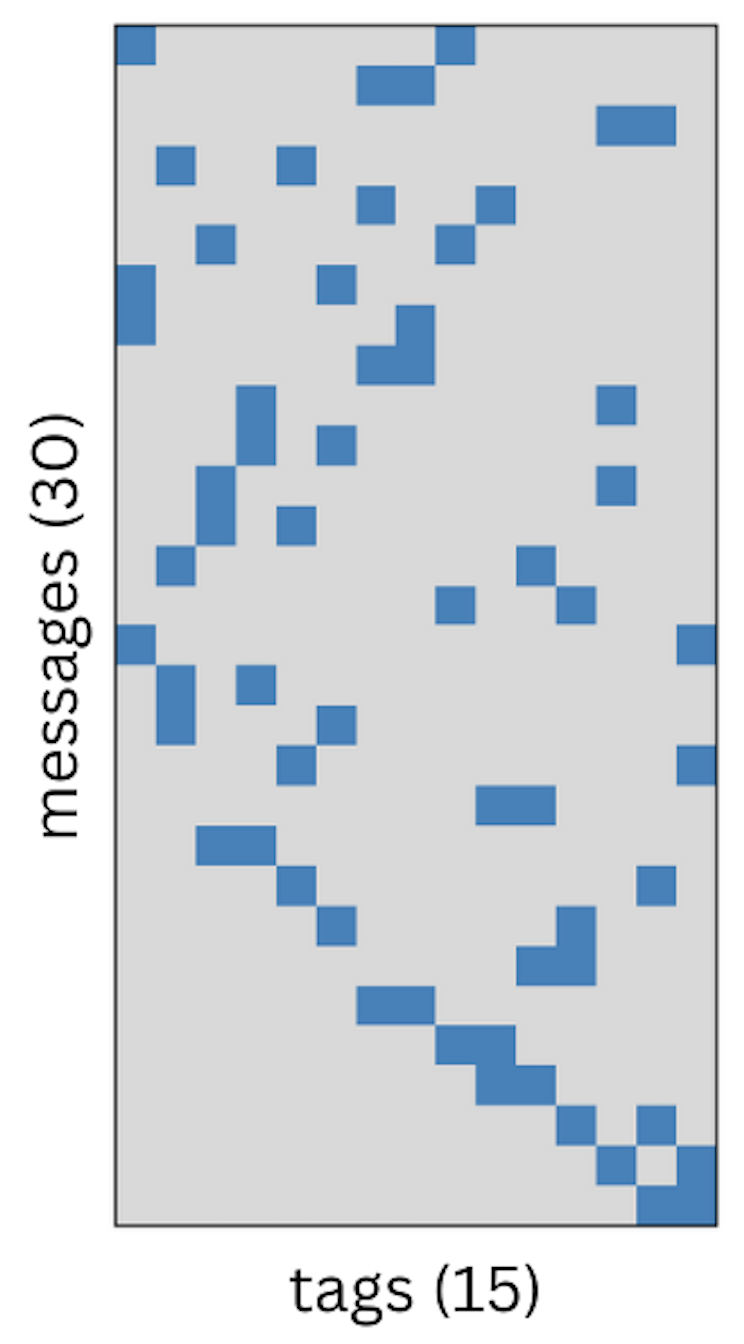
\includegraphics[width=0.38\columnwidth]{img/X.png}
%     \caption{An optimized $X$  matrix of TMR = 15/30.}
%     \label{fig:xmatrix}
% \end{wrapfigure}
 usually depending on the size and the number of tags they generate or transmit per message. However, comparing different schemes' efficiency is difficult, and to simplify comparison, we assume these schemes deploy the same algorithm and generate the same tag size. Based on this assumption, We define TMR ($\frac{n}{m}$), a metric designed to evaluate the efficiency of integrity check schemes, given by:

\begin{equation}
    \frac{n}{m} = \dfrac{\text{total number of tags}}{\text{total number of messages}}
\end{equation}
 
Assuming that transmitting number of tags is less than or equal to the number of messages, $\frac{n}{m}$ provides a normalized value between 0 and 1, where 0 indicates the optimal scenario where no tags are used, representing the highest possible efficiency and 1 indicates that the scheme has no improvement over the traditional method (one tag per message).
\begin{figure}[h]
    \centering
    
\includegraphics[width=.8\linewidth]{img/results/X.png}
    \caption{Two Optimized Matrix \textbf{X} with TMR = 10/25 and 15/25  from left to right, respectability. The yellow squares indicate a 1 representing a message to a tag assignment.}
    \label{fig:placeholder}
\end{figure}





\subsubsection{Tag-bits per Message (TbpM)}
Although Goodput shows the bandwidth efficiency of the MAC schemes, it does not capture the system's security strength. For example, in the Whips shown in Figure~\ref{fig:proMAC}, for every message to achieve a security equal to 258-bit, three tags of size 86 bits are required. However, A packet loss, as shown in equation~\eqref{proMAC_packetLoss_example}, resulted in 9 fewer verifications than expected, equivalent to 774 fewer bits of security overall.

Therefore, we define Tag-bits per Message as follows: 
\begin{equation}\label{tbpm}
    TbpM = \frac{\sum_{i  = 1}^m \sum_{j \in \{j \mid X_{ij} = 1 \} } Pr(U_j=1)|t_j|}{m}
\end{equation}
Assuming that  $|t_j| = |t| \quad \forall j $ we can further simplify the equation above:
\begin{equation}
    TbpM = \frac{|t|\sum_{i  = 1}^m E[A_i]}{m},
\end{equation}
where the tag length is represented by $|t_j|$, and there are in total of $m$ messages.
Equation~\eqref{tbpm}, is the expected number of usable tag bits per message for statistical analysis, however for deterministic analysis , the $Pr(U_j=1)$ must be replaced by $U_j$.

\subsubsection{Authentication Latency (L)}
Packet latency is when a packet is sent and when the integrity check scheme verifies it. Multiple factors influence it, including implementation details, data rates, and computational power. Additionally, the latency can vary depending on the network layer where the integrity check is deployed. Our objective is to specifically assess the impact of the integrity check scheme on latency compared to traditional MACs under both ideal and attack scenarios. It's important to note that underlying layers—such as the physical, data link, and transport layers—can also contribute to latency, especially when the system is under attack.

To facilitate a relative comparison with traditional MACs, we assume that all tags and messages are correctly received. Under this assumption, authentication latency is the number of additional messages that must be received before a specific message can be authenticated, assuming messages are transmitted sequentially. For instance, if tag $t_j$ verifies messages \( m_{i+1}, m_{i+3}, m_{i+7} \) then \( m_{i+1}\) can be verified only after \( m_{i+\{2,\cdots,7\}} \) are received, which by our definition, the latency is six.

Let's assume that all the messages are sent in order based on their index. For example, \( m_1 \) is sent first and \( m_2 \) is sent afterward. We define the Tag Maximum Index (\textbf{TMI}) vector, where the \( j \)-th entry is the maximum index of the message that the tag \( t_j \) is verifying.
\begin{equation}
	TMI_j= \max_{i \in \{i \mid X_{ij} = 1\}} i 
\end{equation}

For example, in the compound MAC shown in Fig.~\ref{fig:compoundMAC}, \( TMI_{j+2} \) corresponding to tag \( t_{j+2} \) equals \( i+6 \), since the the messages that are verified by tag \( t_{j+2} \) are \( m_{i+4}, m_{i+5}, \text{ and } m_{i+6}\).
The authentication latency vector \( \textbf{L} \) is defined as follows:
\begin{equation}
	L_i = 
	\begin{cases} 
		\left(\min_{j \in \{j \mid X_{ij}=1 \}} TMI_j \right)-i & \text{if } A_i > 0 \\
		\text{penalty} & \text{otherwise}
	\end{cases}
\end{equation}
The penalty is the value assigned if message \( m_i \) is not verified by any tag. For example, the latency vector for the Progressive MAC is all zeros. However, the latency vector for the Compound MAC will be as follows:
$$L = [2, 1, 0, 2, 1, 0, \cdots]$$

\subsubsection{Strength Number (SN)}
The Strength number SN represents the smallest ratio of messages or tags that, if lost, would prevent the verification of all messages. An upper bound for the strength number is the total number of tags divided by the number of messages, as destroying all tags would result in no verifiable message. If the set consists only of tags, it must include all tags to ensure no message can be verified. However, any tag within this set can be replaced by a message it verifies. If tag-to-message substitutions are selected strategically in a way that for at least two tags, a common message is replaced, the resulting set can potentially have a cardinality less than the number of tags.

Thus, the strength number can be formulated as the minimum number of messages that will make all the tags unusable divided by the number of messages. As a result, let \( \textbf{S} \subseteq \{m_1, m_2, \ldots, m_m\} \) and for any tag, there exists a message in SN that is verified by that tag. 
\begin{equation}
	\textbf{S} = \left\{m_i \mid \quad \forall j, \exists i \quad \text{such that} \quad X_{ij}=1 \right\} 
\end{equation}
The $|\textbf{S}|$ must be minimized to find the strength number. 
% This can be achieved by finding the minimum set of rows in the \( X \) matrix that, when summed, produces a row with all elements greater than or equal to one. To compare different schemes, \( |\textbf{S}| \) can be divided by the total number of messages \( |M| \) to be normalized.
For a given matrix $X$, finding the strength number is similar to the classical set covering the problem with the following formulation. We define a binary variable \( s_i \) for each message.
\begin{equation}
	s_i =
	\begin{cases} 
		1 & \text{if message $i$ is selected} , \\
		0 & \text{otherwise}.
	\end{cases}
\end{equation}
The mathematical formulation of this set covering problem will be as follows:
\begin{align}
	& \text{min} \sum_{i=1}^{m} s_i  &&  \\
	& \text{subject to}&& \nonumber\\
	& && \sum_{i \in \{i| X_{ij}=1\}} s_i \geq 1, \quad \forall j \in \{1, 2, \ldots, n\} \label{setCoveringConstraint} \\
	& && s_i \in \{0, 1\}, \quad \forall i \in \{1, 2, \ldots, m\}
\end{align}
In this formulation, the constraint~\eqref{setCoveringConstraint} guarantees no message will be verified. The objective function is of type cardinality, effectively counting the minimum possible number of messages that guarantee the total failure of the system. Note that the constraint~\eqref{setCoveringConstraint} should only be used for the active tags in $X$.  Further, $|S|$ must be normalized by the number of messages. Therefore $SN$ is given by:
\begin{equation}
	SN = \dfrac{\text{min}(|S|)}{m},
\end{equation}
where $m$ is the number of messages. The strength number effectively measures the security in terms of availability, representing the percentage of packet loss that results in system failure.
\begin{figure}[h]
	\centering
	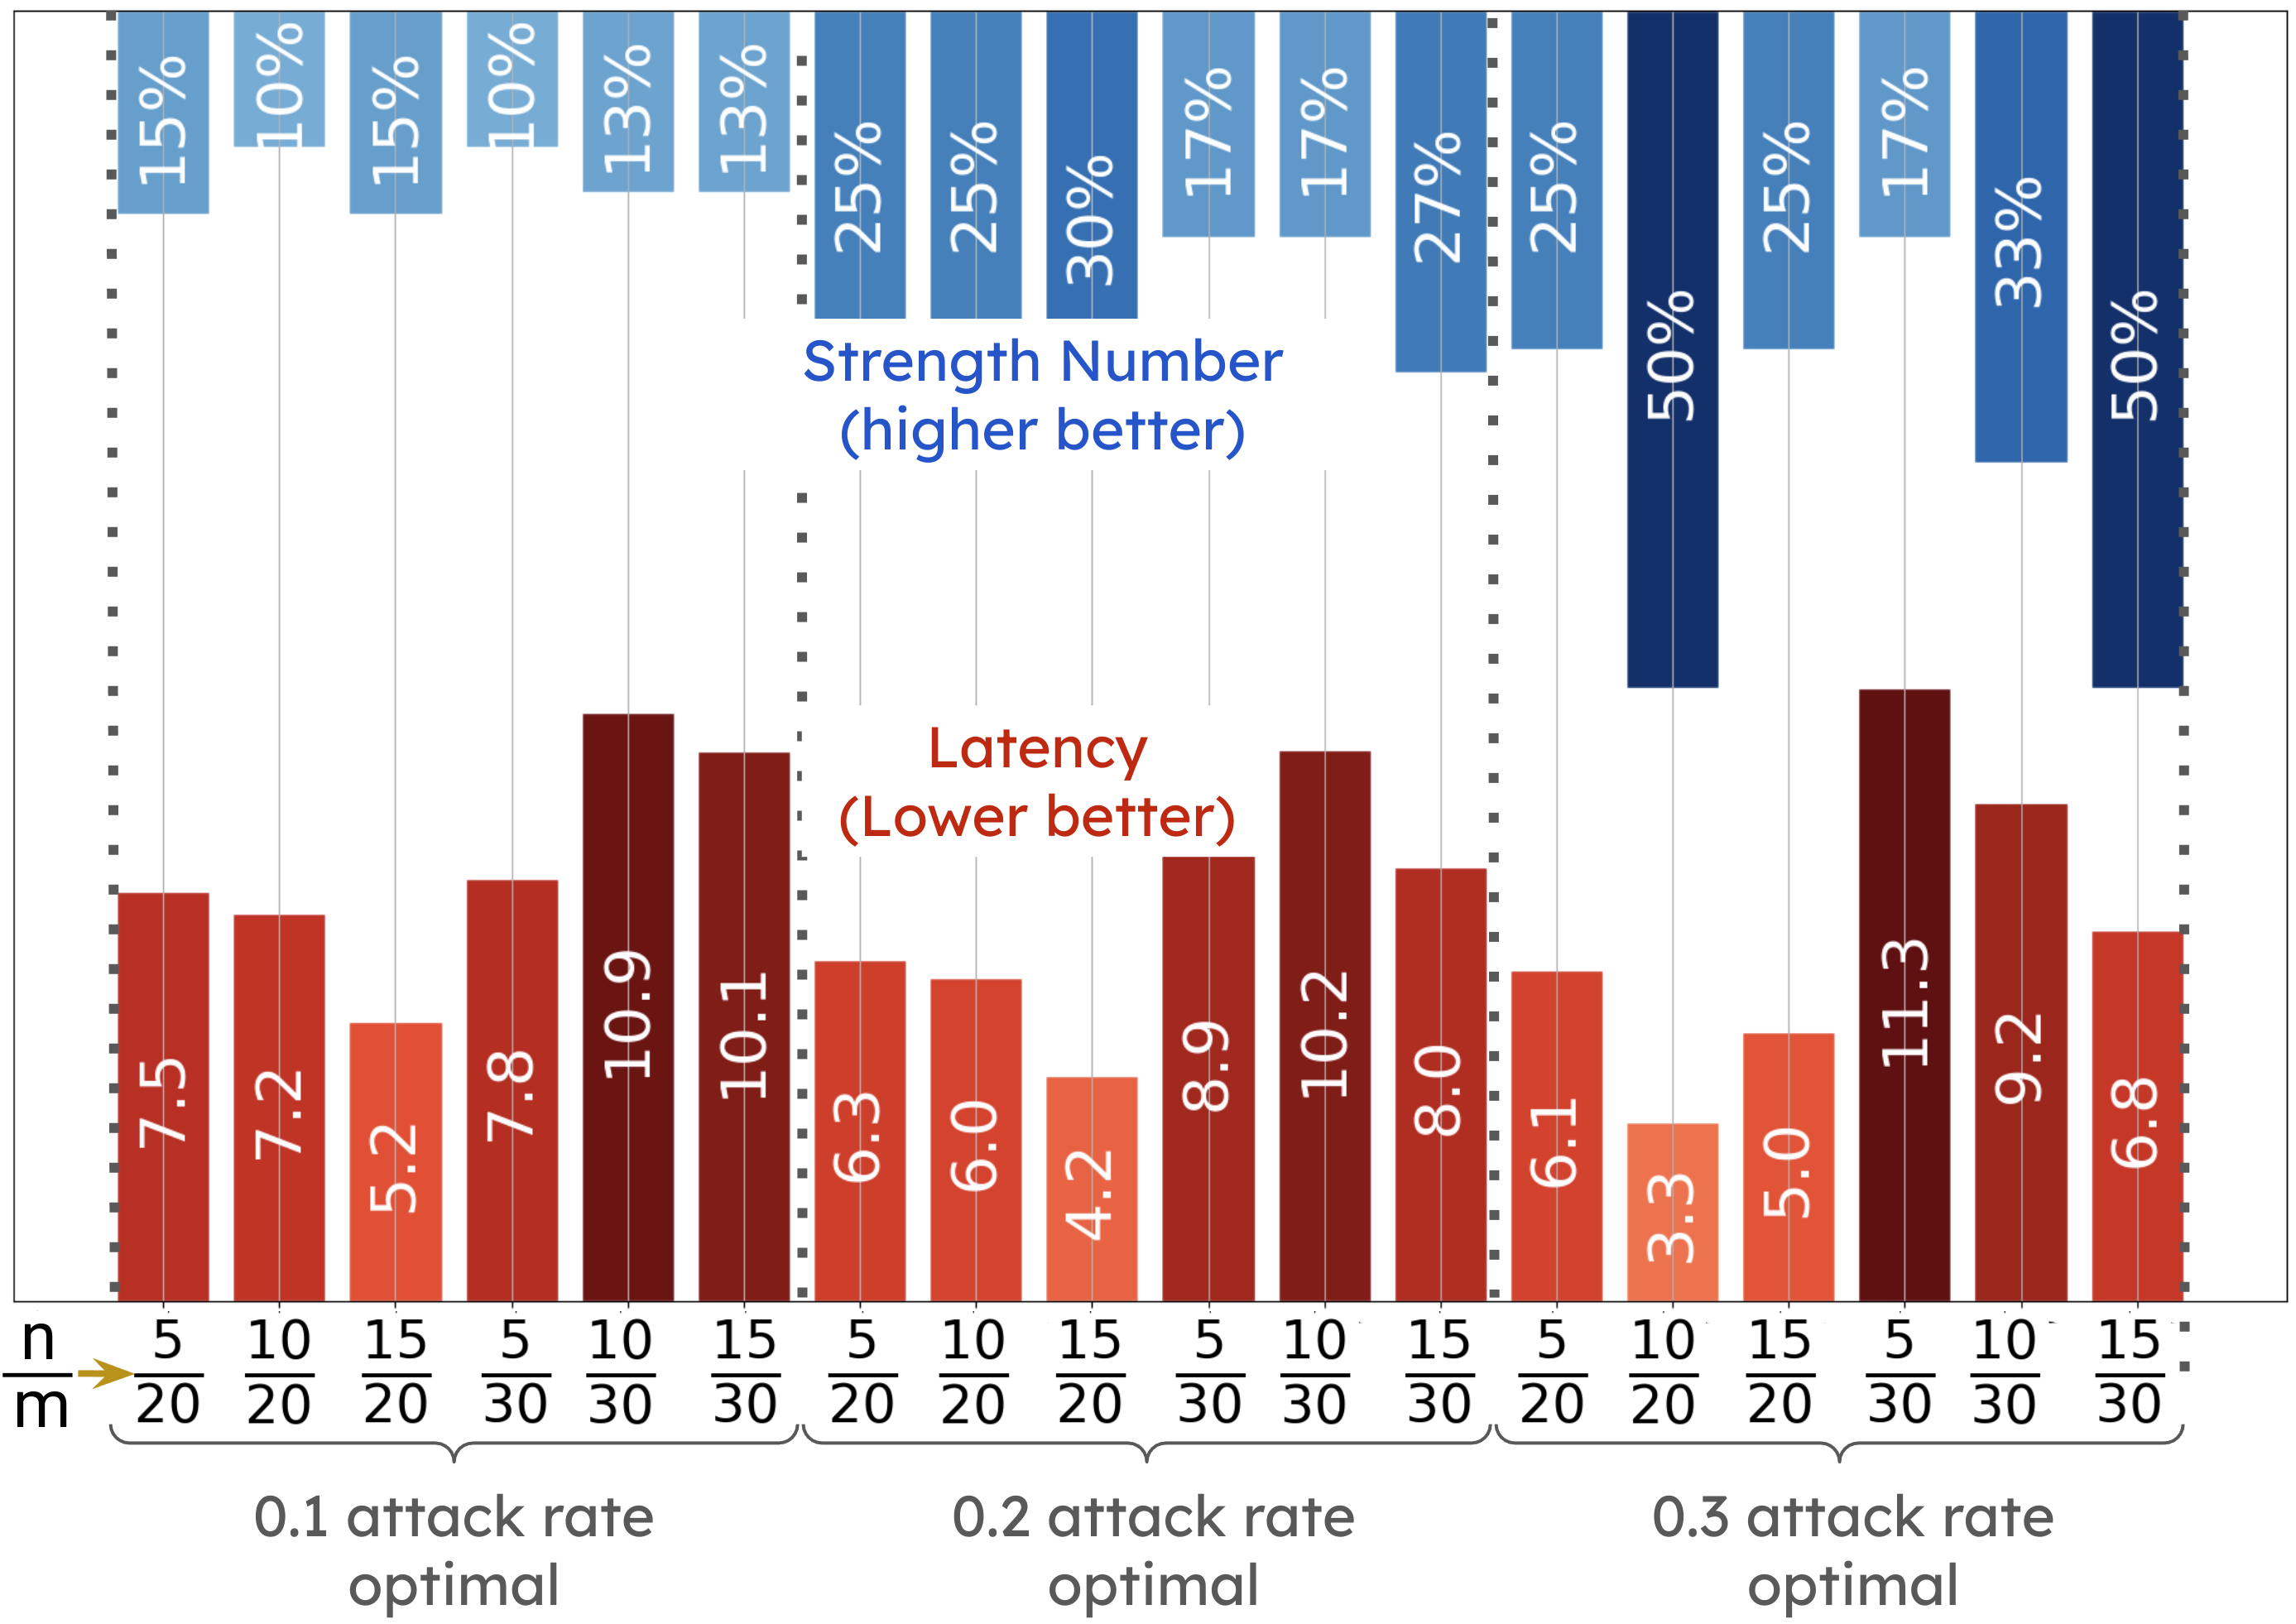
\includegraphics[width=.9\columnwidth]{img/results/SN vs Latency.png}
	\caption{Strength Number and Latency for the optimal solution by attack rates and Tag-to-Message Ratio ($\frac{n}{m}$).}
	\label{fig:otehrMetrics}
\end{figure}
Figure~\ref{fig:otehrMetrics} provides a comparative analysis of the effects of the optimization model on Strength Number (SN) and Latency (L) across different configurations optimized for three distinct attack rates: 0.1, 0.2, and 0.3. Each section corresponds to a specific attack rate and displays bars representing the values of SN (in blue) and L (in red) for various schemes, where each scheme is characterized by a different TMR \( n/m \).


%\subsection{Simulation under Periodic Jamming}
%
%We simulated the transmission of $100{,}000$ packets under periodic jamming,
%where every other message is dropped with probability $p$. Each packet carries
%a $32$-bit message, and the tag sizes were optimized to satisfy a $256$-bit
%security requirement. Figure~\ref{fig:periodic} illustrate the goodput of prior scheme compared to OptiMAC.
%\begin{figure*}
%	\centering
%	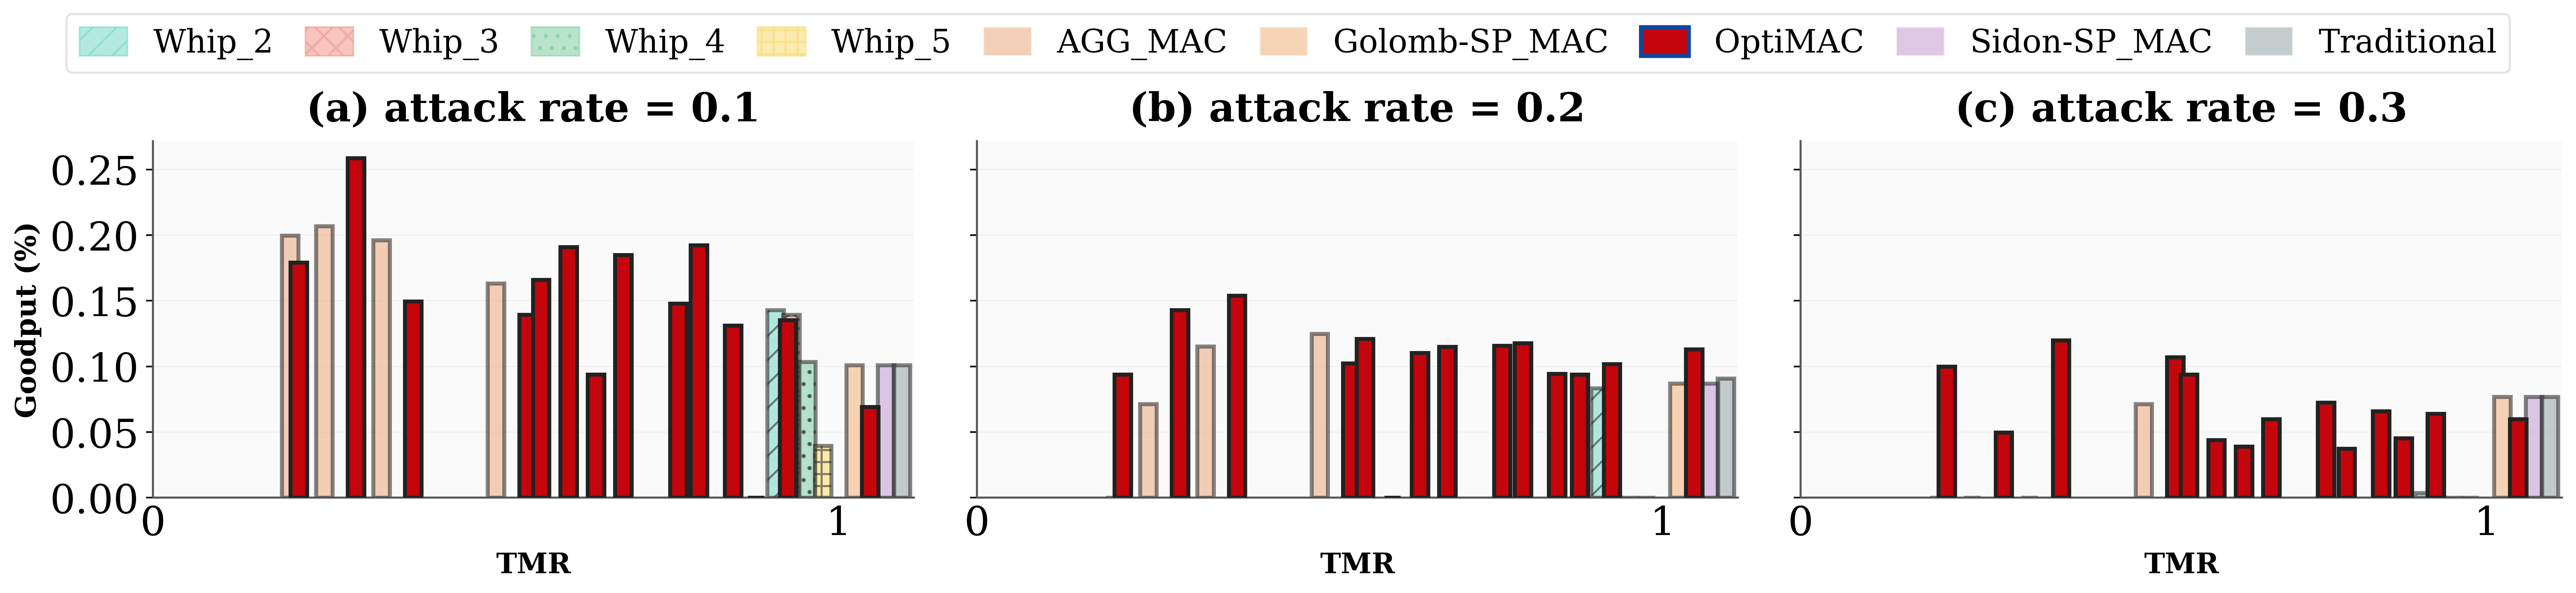
\includegraphics[width=.95\linewidth]{img/output2.png}
%	\caption{Periodic jamming simulation for message size of 32 bits and security requirements of 256 bits. OptiMAC is the only scheme that can provide adaptive solutions for TMR between 1/2 and 1.}
%	\label{fig:periodic}
%\end{figure*}
%
%The results highlight several key observations. First, most prior schemes are
%restricted to a TMR of exactly one (Traditional, WHIP variants, ...), meaning that every message must be accompanied by a tag. aggregate MAC partially relaxes this by offering ratios of $1/n$, but still only at fixed discrete points. By contrast, OptiMAC supports \emph{arbitrary} TMR values, enabling a much finer adjustment between security and throughput. This flexibility translates into higher goodput across a wide range of $p$ values, particularly under severe jamming conditions ($p=0.6,0.7$), where OptiMAC consistently achieves the best
%performance among all schemes.



\subsection{Real-world Testbed}
We have created two real-world testbeds to evaluate the impact of packet interference on webcam video streaming using the UDP protocol on WiFi and 5G networks. The interference sources included an attacker modifying packet data. The objective is to assess the impact on transmission integrity and performance metrics, particularly under adverse conditions.

\subsubsection{WiFi Testbed Setup}
The experimental setup involved a host machine connected to a Logitech HD Pro C920 X webcam, which captured real-time video frames at a resolution 1080p and a frame rate of 30 fps. These frames were transmitted over a WiFi network using the UDP protocol. The UDP packets were customized by appending additional tags according to matrix \textbf{X}.

The transmitter was equipped with an Intel WiFi 6 AX200 (rev 1a) adapter, configured on a Linux Ubuntu 24.04 LTS system with an Intel Core i7-11700K processor. The WiFi hotspot was managed using the nmcli tool, configured to operate on the 802.11 bg at 2.4 GHz band. The video data was encoded using JPEG Progressive format, with varying quality settings 25\% corresponding to data 650  KB/s rate.

% A WiFi jammer was introduced to the experimental setup to simulate signal interference. The jammer hardware consisted of USRP B210 Software Defined Radios (SDRs) and VERT2450 antennas. The WiFi protocol uses Carrier Sense Multiple Access with Collision Avoidance (CSMA/CA) to avoid packet collisions~\cite{wang2006csma}, which means simple constant jamming is not ideal. Therefore a jammer needs to avoid the WiFi protocol's avoidance mechanism to disrupt the transmission by performing random or periodic jamming. This was achieved using Pulse Width Modulation (PWM), with a PWM setting of 10\%. Moreover, there were two different gain settings for the SDR emulating two different jam-to-signal ratios. At the same time, the PWM determines the proportion of time the jammer is active, enabling it to disrupt the transmission and drop packets effectively. The jammer was activated halfway through the experiment to observe its effects on the transmission metrics. It is worth mentioning that the insider attack in our testbed can easily modify and prevent the packet from being sent without any knowledge about other layers and implementation. 

\subsubsection{5G Testbed Setup}
We set up the 5G testbed using an open-source 5G software stack. We use the User Equipment (UE) and gNodeB implementation from OpenAirInterface \cite{oai} and the 5G Core Network from Open5GS \cite{open5gs}. 

The experiment runs on two host machines. Both machines run Ubuntu 22.04 LTS with Intel Core i9-14900K and 64 GB of memory. Host 1 is equipped with 1 USRP B210 software-defined radio and runs the UE 1. Host 2 is equipped with 2 USRP B210s and runs the gNodeB, UE 2, and the 5G Core.  

In our setup, Host 1 acts as the sender. It captures real-time video frames from a Logitech C930e webcam and sends the UDP packets to UE software. The UE 1 running on the same machine receives the packets, processes them in the 5G stack, and sends the data over-the-air to the gNodeB. The gNodeB in Host 2 receives the data from UE 1 and sends it to the Core Network for routing to UE 2. Then, the Core Network routes the packets from the gNodeB over-the-air to the UE 2. Our receiver listening on UE 2 finally receives the transmitted data frame. 
% \yilu{should I draw a figure?}

% Due to the capacity of these software implementations, we can only achieve [list the packet parameters] \yilu{do we need to mention this?}\moh{I don't think so!}

\subsubsection{Transmission Setup}
The transmitted data was structured at the application layer with a custom frame format. Each frame included a 4-byte sequence number, an 8-byte timestamp, and a variable-length data field. 

\renewcommand{\arraystretch}{1.9}

\begin{table}[h!]
\centering
\caption{Experiment parameters for WiFi and 5G}
\label{tab:setting}
\begin{tabular}{c|c|c|c|}
\cline{2-4}
% & \begin{tabular}[c]{@{}c@{}}Data Rate\\ (KB/S)\end{tabular} 
% & \begin{tabular}[c]{@{}c@{}}Payload Size\\ (Bytes)\end{tabular} 
% & \begin{tabular}[c]{@{}c@{}}Tag length\\ (Bytes)\end{tabular} 

&\begin{tabular}{c}
     Data Rate  \\
     (KB/S) 
\end{tabular}   & 
\begin{tabular}{c}
    Message Size\\ 
    (bits) 
\end{tabular}   & 
\begin{tabular}{c}
    Tag length \\
    (bits)
\end{tabular}
\\ \hline 


\multicolumn{1}{|c|}{\textbf{ 5G}}   & 300  & 768 & 512    \\ \hline
\multicolumn{1}{|c|}{ \textbf{WiFi}} & 600  & 128  & 256   \\ \hline
\end{tabular}
\end{table}

\setlength{\tabcolsep}{1.9pt}




The data was then transmitted using the UDP/IP transport layer, to avoid further influence of the transportation layer. The details of the setup configuration for each setting are as follows. To accommodate flexibility to perform integrity checks for any given matrix \textbf{X}, an increase in the complexity of the implementation was necessary. This complexity arose from the need to manage multiple packets before the integrity check was possible, which was achieved by utilizing a book-like buffer structure. In this structure, each "page" holds a certain number of packets based on matrix \textbf{X} dimensions. Once a page is full, it is processed and then released. Although this approach required a larger buffer and introduced additional complexity, we were able to demonstrate that it was manageable by successfully implementing and testing live video streaming at different data rates both in the WiFi and 5G testbed.

The impact of an attacker modifying packets on video transmission was assessed using several key metrics: the number of bits verified per message ($TbpM$), and goodput ($G$). Accurately measuring latency posed a challenge due to the need for precise synchronization between the two devices; therefore, we acknowledge that the latency measurements was not entirely accurate. However, in the future we will try to incorporate a mechanism to reliably measure the latency.







\section{Results}\label{Discussion}




In this section, we analyze the trade-off between security, goodput, and latency achieved by various MAC schemes based on their tag sizes and tag-to-message ratios (TMR).
The tag-bits per message (TbpM) is a metric used to measure the integrity and availability of the system. Moreover, Goodput and TMR are metrics to show both the bandwidth and energy efficiency of the system.. 


\subsection{Computation and Latency Overhead}

To evaluate latency and computational overhead of different MAC schemes, we use an application-level metric based on real-time video streaming. Specifically, we measure the number of successfully verified frames per second (FPS) in our 5G experimental testbed, as shown in Fig.~\ref{fig:fps}. Since the camera generates frames at a fixed rate of 30 FPS, the achieved FPS reflects the system’s ability to process, authenticate, and verify packets in real time. Therefore, FPS serves as a practical proxy for both computational overhead and end-to-end latency.

\begin{figure}[h!]
	\centering
	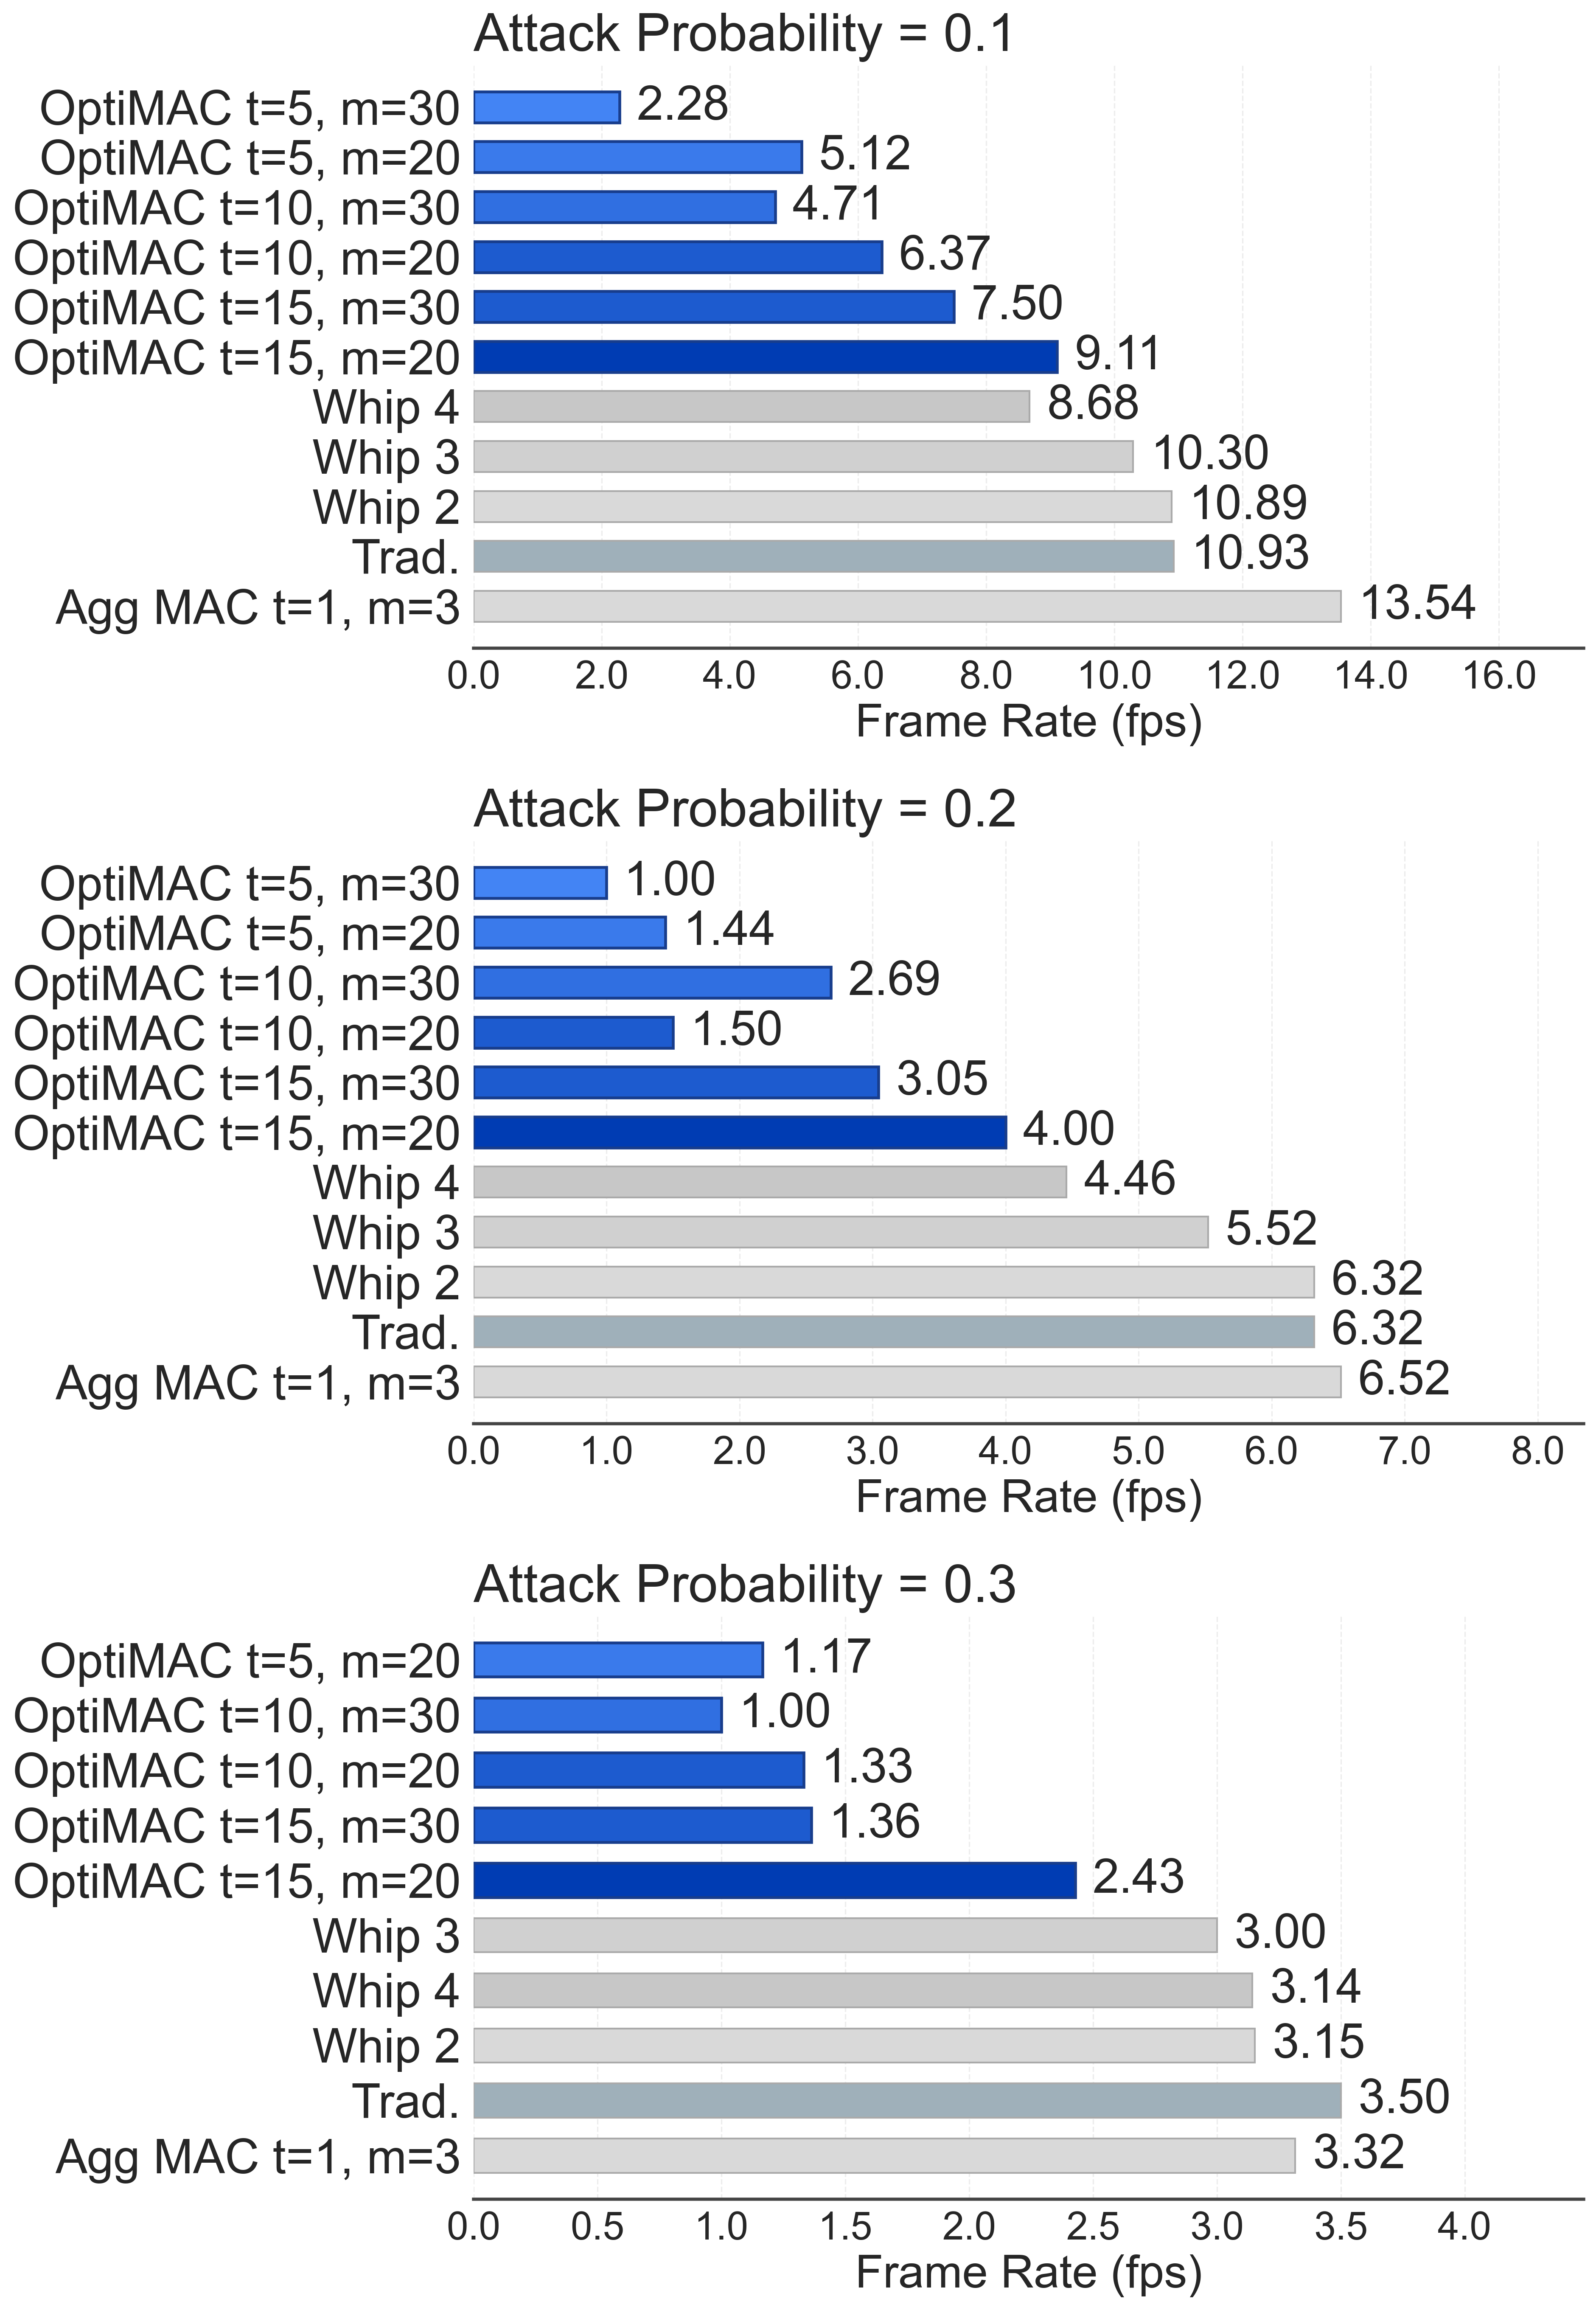
\includegraphics[width=\linewidth]{img/results/FrameRate.png}
	\caption{Frame rate (FPS)  under varying attack probabilities }
	\label{fig:fps}
\end{figure}

Fig.~\ref{fig:fps} shows the achieved frame rates under different attack probabilities (0.1, 0.2, and 0.3). As the attack probability increases, all schemes exhibit a reduction in FPS. This degradation is primarily due to increased packet loss, which limits the number of successfully verified packets available for frame reconstruction. In our implementation  correct decoding requires the availability of critical header and payload data. When a sufficient number of packets cannot be verified, the decoder fails to reconstruct the frame, resulting in dropped frames and a corresponding reduction in FPS. Furthermore, as the dependency matrix size increases, the authentication process becomes more complex, leading to higher authentication latency (L). This effect is evident when comparing different OptiMAC configurations, where smaller matrices (e.g., $t{=}10, m{=}20$) achieve higher FPS than larger ones (e.g., $t{=}15, m{=}30$) due to reduced verification delay. Therefore, the observed decrease in FPS reflects not only increased computational and communication overhead, but also the impact of both insufficient verified data and higher authentication latency under adversarial conditions.

Our prototype is implemented in Python at the application layer and is not optimized for performance. Nevertheless, OptiMAC supports real-time streaming at practical frame rates. A production-level implementation (e.g., in C/C++ or at the data link layer) is expected to further reduce overhead and latency. 

\subsection{Tag-bit per Message (TbpM) vs Goodput}
Similar to progressive MAC~\cite{ProMAC1}, adjusting the tag bits per message could be advantageous in balancing the overhead trade-off. A higher TbpM allows for shortening the tag length while satisfying the security requirements. However, in lossy channels, where the expected number of verifications is lower than in error-free channels, shortening the tag must be done carefully. 
\begin{wrapfigure}{l}{0.6\linewidth}
	\centering
	
\includegraphics[width=\linewidth]{img/results/WiFi/0.1SG.png}
	\caption{TbpM vs. Goodput for WiFi where a 256-bit tag was used (above 128 bits is considered as high security) under 0.1 attack rate.}
	\label{fig:explaing}
\end{wrapfigure}
For a MAC scheme to be considered secure, it must maintain a tag size of at least 64 bits, as per NIST standards~\cite{nist_64bits}. However, NIST emphasizes the actual tag length that may vary depending on the specific algorithm employed, and some applications, like IPsec, mandate a minimum of 128-bit tags without truncation to ensure robust security~\cite{nist_gcm_update}. Without loss of generality, In the rest of this paper, we assume more than 128 and 256 Tag-bits per Message (TbpM) are high security for WiFi and 5G, respectively.

In our study, any scheme with TMR exceeding the threshold set by the aggregate MAC scheme (i.e., one tag per two messages) is a high TMR scheme. Low TMR schemes are expected to offer more efficient bandwidth and computational usage by lowering the number of tags transmitted, though this may impact security if not managed carefully. By comparing various approaches in terms of security (measured in TbpM), we demonstrate the potential of optiMAC schemes to balance these factors, particularly in adversarial environments.

The results, visualized in Figure~\ref{fig:explaing}, illustrate that optiMAC (indicated in blue) generally outperforms state-of-the-art methods (in red) by achieving both high security and goodput.  The figure is divided into quadrants with shaded regions to indicate different trade-offs. The green area represents methods that achieve best in both metrics. The blue and light pink areas highlight methods that emphasize one metric but have sacrificed the other. The red area shows methods with both metrics are low, making these methods less desirable. By comparing the positions of red and blue points, it can be observed the relative performance of different methods. Blue points often appear in the green quadrant, suggesting a favorable balance between the metrics. 
%\begin{figure*}[h]
%     \centering
%          \begin{subfigure}[b]{0.32\linewidth}
%         \centering
%         
\includegraphics[width=\linewidth]{img/results/WiFi/0.1S'.png}
%         \caption{Attack rate 0.1}
%         \label{fig:0.1S WiFi}
%     \end{subfigure} \hfill
%     \begin{subfigure}[b]{0.32\linewidth}
%         \centering
%         
\includegraphics[width=\linewidth]{img/results/WiFi/0.2S'.png}
%         \caption{Attack rate 0.2}
%         \label{fig:0.2S WiFi}
%     \end{subfigure}
%     \hfill
%      \begin{subfigure}[b]{0.32\linewidth}
%         \centering
%         
\includegraphics[width=\linewidth]{img/results/WiFi/0.3S'.png}
%         \caption{Attack rate 0.3}
%         \label{fig:0.3S WiFi}
%     \end{subfigure}
%
%     \caption{TbpM (y-axis) vs. TMR (x-axis) of WiFi experiments with 256-bit tags (128 or higher TbpM is high security). State-of-the-art (SOTA) includes traditional, progressive, and aggregate MAC vs. the optimal by optiMAC.}
%     \label{fig:SecurityWiFi}
%\end{figure*}
%\begin{figure*}[h]
%     \centering
%          \begin{subfigure}[b]{0.32\linewidth}
%         \centering
%         
\includegraphics[width=\linewidth]{img/results/WiFi/0.1G'.png}
%         \caption{Attack rate 0.1}
%         \label{fig:0.1G WiFi}
%     \end{subfigure} \hfill
%     \begin{subfigure}[b]{0.32\linewidth}
%         \centering
%         
\includegraphics[width=\linewidth]{img/results/WiFi/0.2G'.png}
%         \caption{Attack rate 0.2}
%         \label{fig:0.2G WiFi}
%     \end{subfigure}
%     \hfill
%      \begin{subfigure}[b]{0.32\linewidth}
%         \centering
%         
\includegraphics[width=\linewidth]{img/results/WiFi/0.3G'.png}
%         \caption{Attack rate 0.3}
%         \label{fig:0.3G WiFi}
%     \end{subfigure}
%
%     \caption{Goodput (y-axis) vs. TMR (x-axis) of WiFi experiments where more than 80\% of Traditional MAC's Goodput is considered high. State-of-the-art (SOTA) includes traditional, progressive, and aggregate MAC vs. the optimal by optiMAC.}
%     \label{fig:GoodputWiFi}
%\end{figure*}
Each data point in the figure represents a specific method or configuration. Red points indicate state-of-the-art (SOTA) methods, while blue points represent the optiMAC model. The labels adjacent to the points (e.g., ProMAC and Agg MAC) correspond to different methods, and the accompanying values denote the tag-to-message ratio (TMR). For instance, a TMR of 0.9 implies that for every 10 messages, there are 9 tags, highlighting the balance between security and overhead. As shown in Figure~\ref{fig:explaing}, the Aggregate MAC achieves high security and the highest goodput. On the other hand, optiMAC offers enhanced security with only a slight reduction in goodput (Pareto optimal), demonstrating the trade-off between these factors. This flexibility allows our model to adapt to the specific requirements of various applications, even under adversarial scenarios.

\subsection{Security and Goodput vs TMR}

\begin{figure*}[h]
	\centering
	\begin{subfigure}[b]{0.32\linewidth}
		\centering
		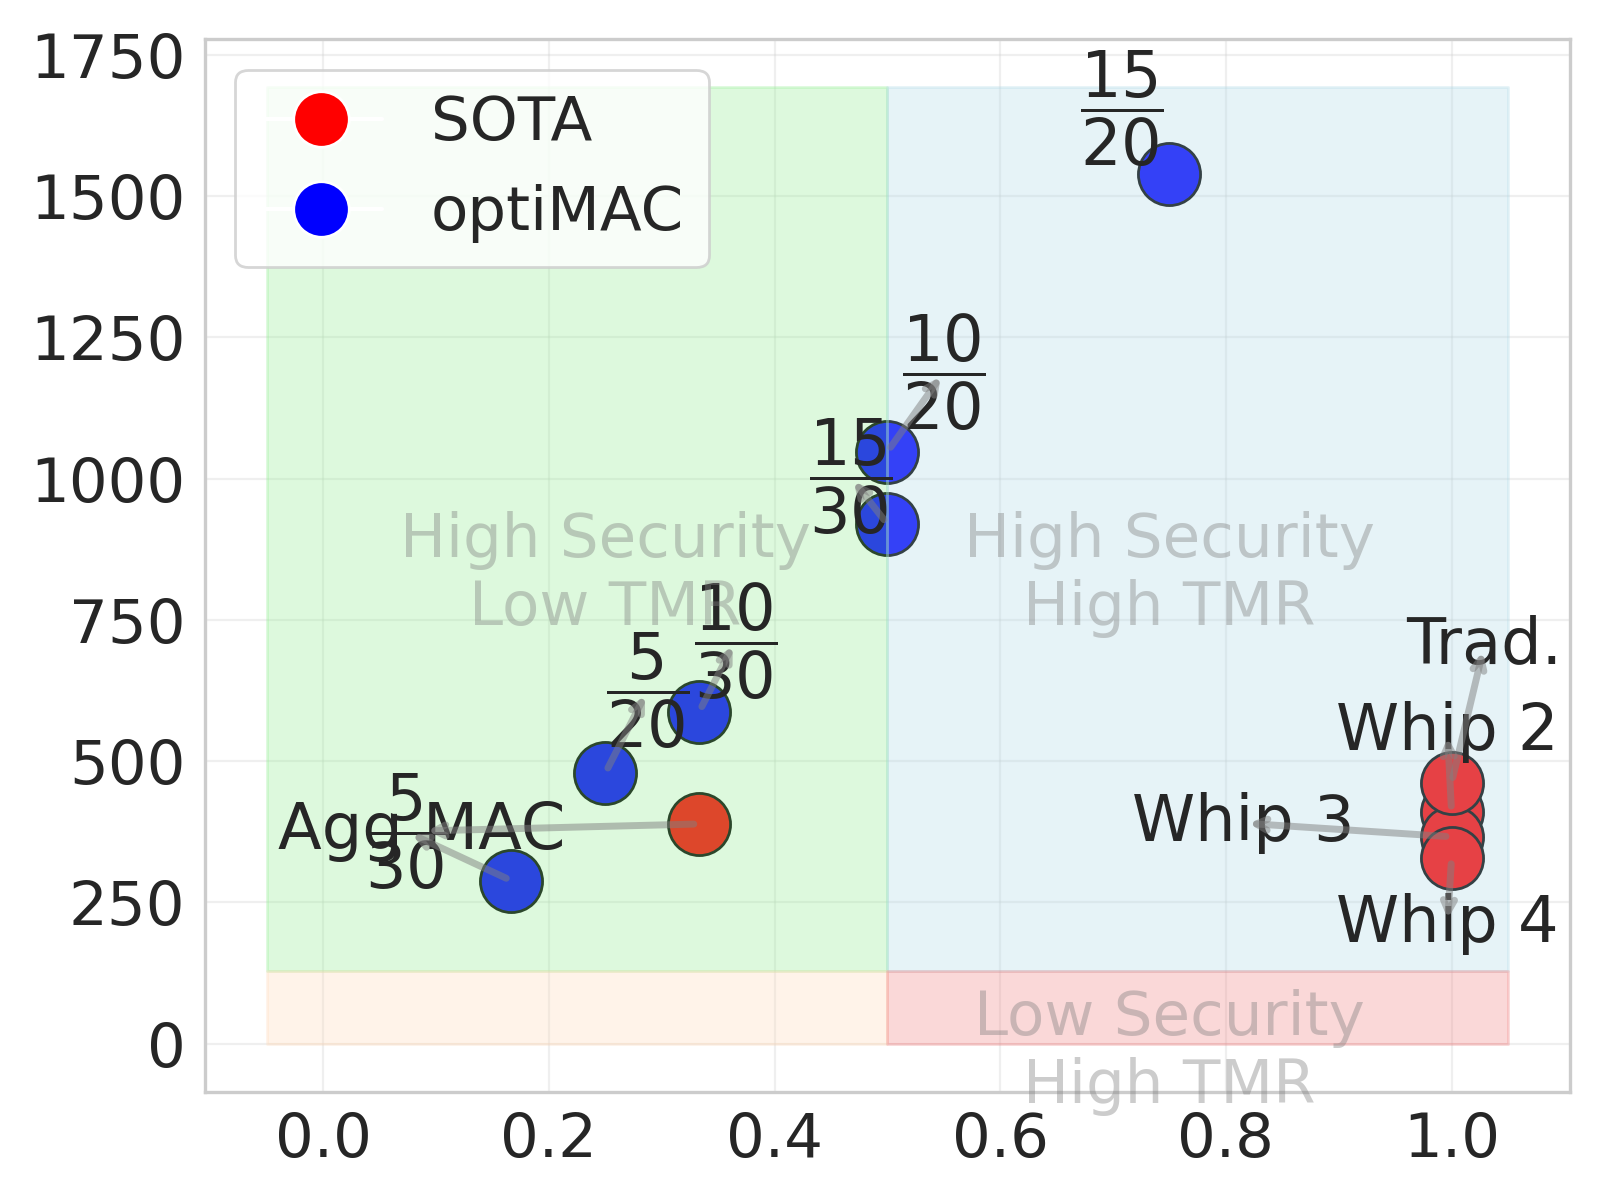
\includegraphics[width=\linewidth]{img/results/5G/0.1S'.png}
		\caption{Attack rate 0.1}
		\label{fig:0.1S 5G}
	\end{subfigure} \hfill
	\begin{subfigure}[b]{0.32\linewidth}
		\centering
		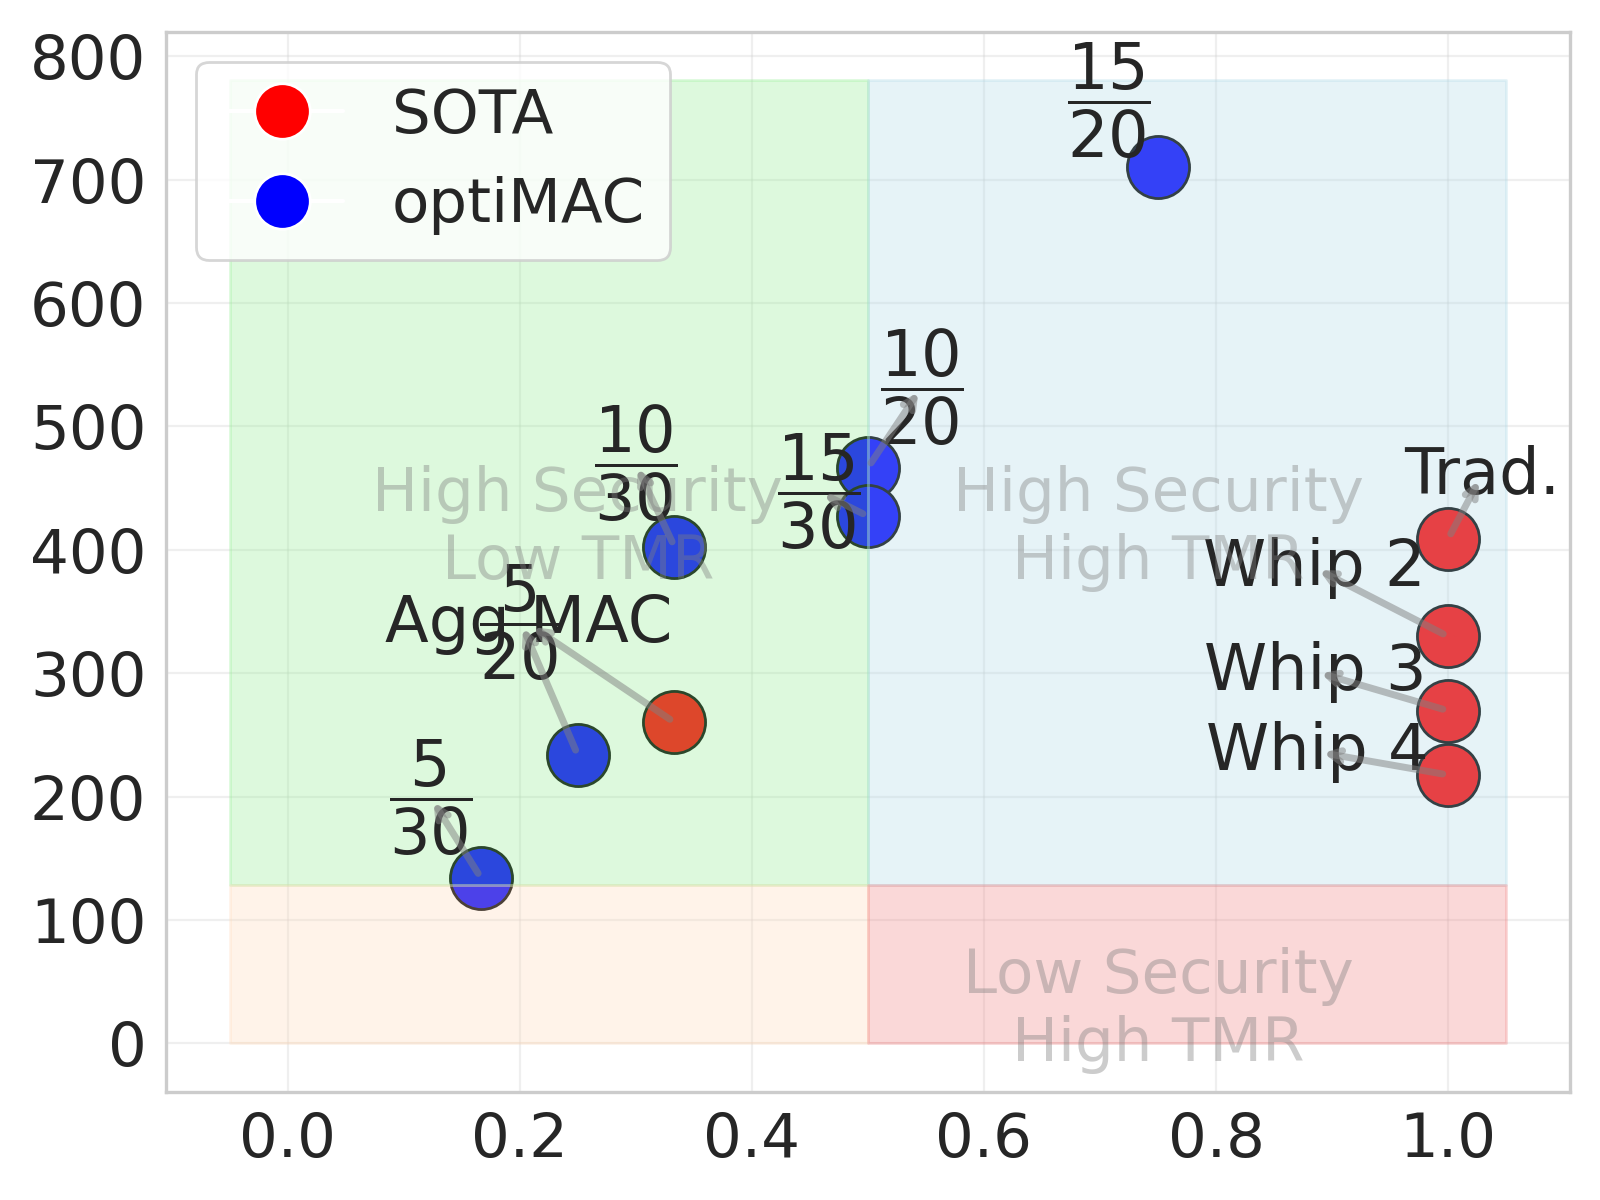
\includegraphics[width=\linewidth]{img/results/5G/0.2S'.png}
		\caption{Attack rate 0.2}
		\label{fig:0.2S 5G}
	\end{subfigure}
	\hfill
	\begin{subfigure}[b]{0.32\linewidth}
		\centering
		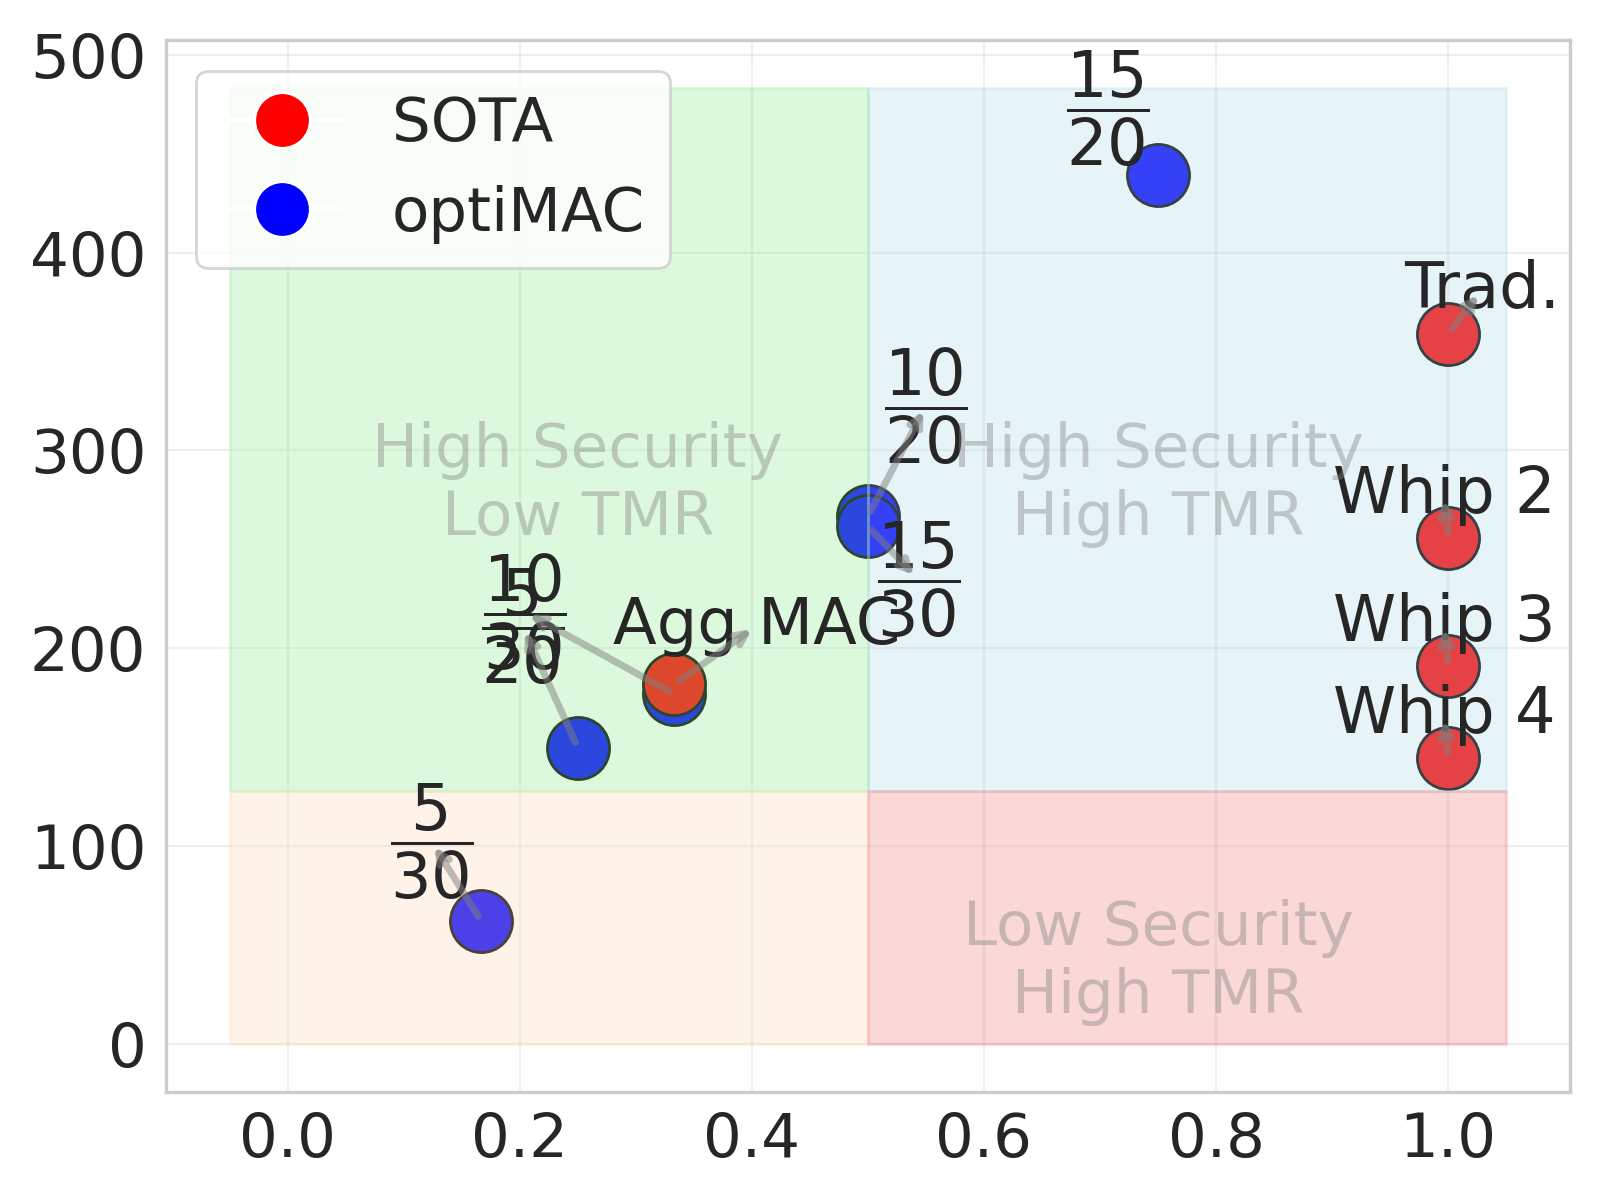
\includegraphics[width=\linewidth]{img/results/5G/0.3S'.png}
		\caption{Attack rate 0.3}
		\label{fig:0.3S 5G}
	\end{subfigure}
	
	\caption{TbpM (y-axis) vs. TMR (x-axis) of 5G experiments with 512-bit tags (256 or higher TbpM is high security). State-of-the-art (SOTA) includes traditional, progressive, and aggregate MAC vs. the optiMAC.}
	\label{fig:Security5G}
\end{figure*}

\begin{figure*}[h]
	\centering
	\begin{subfigure}[b]{0.32\linewidth}
		\centering
		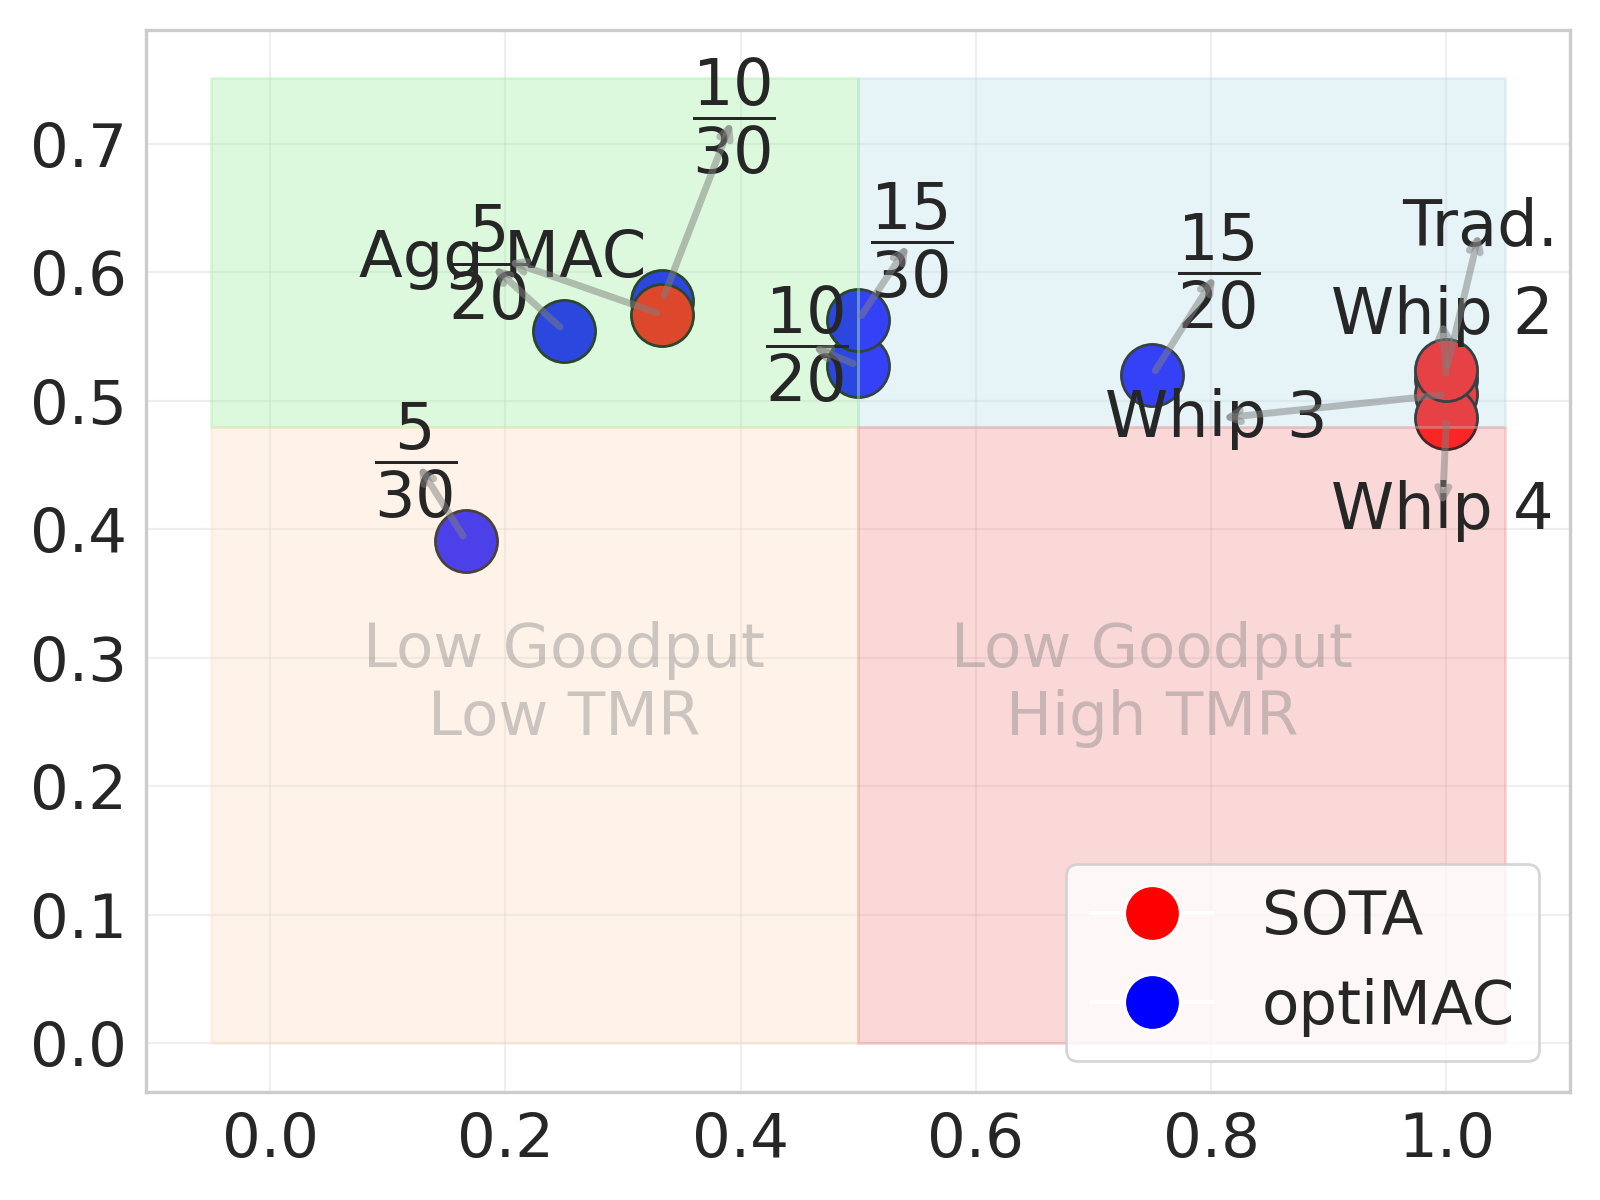
\includegraphics[width=\linewidth]{img/results/5G/0.1G'.png}
		\caption{Attack rate 0.1}
		\label{fig:0.1G 5G}
	\end{subfigure} \hfill
	\begin{subfigure}[b]{0.32\linewidth}
		\centering
		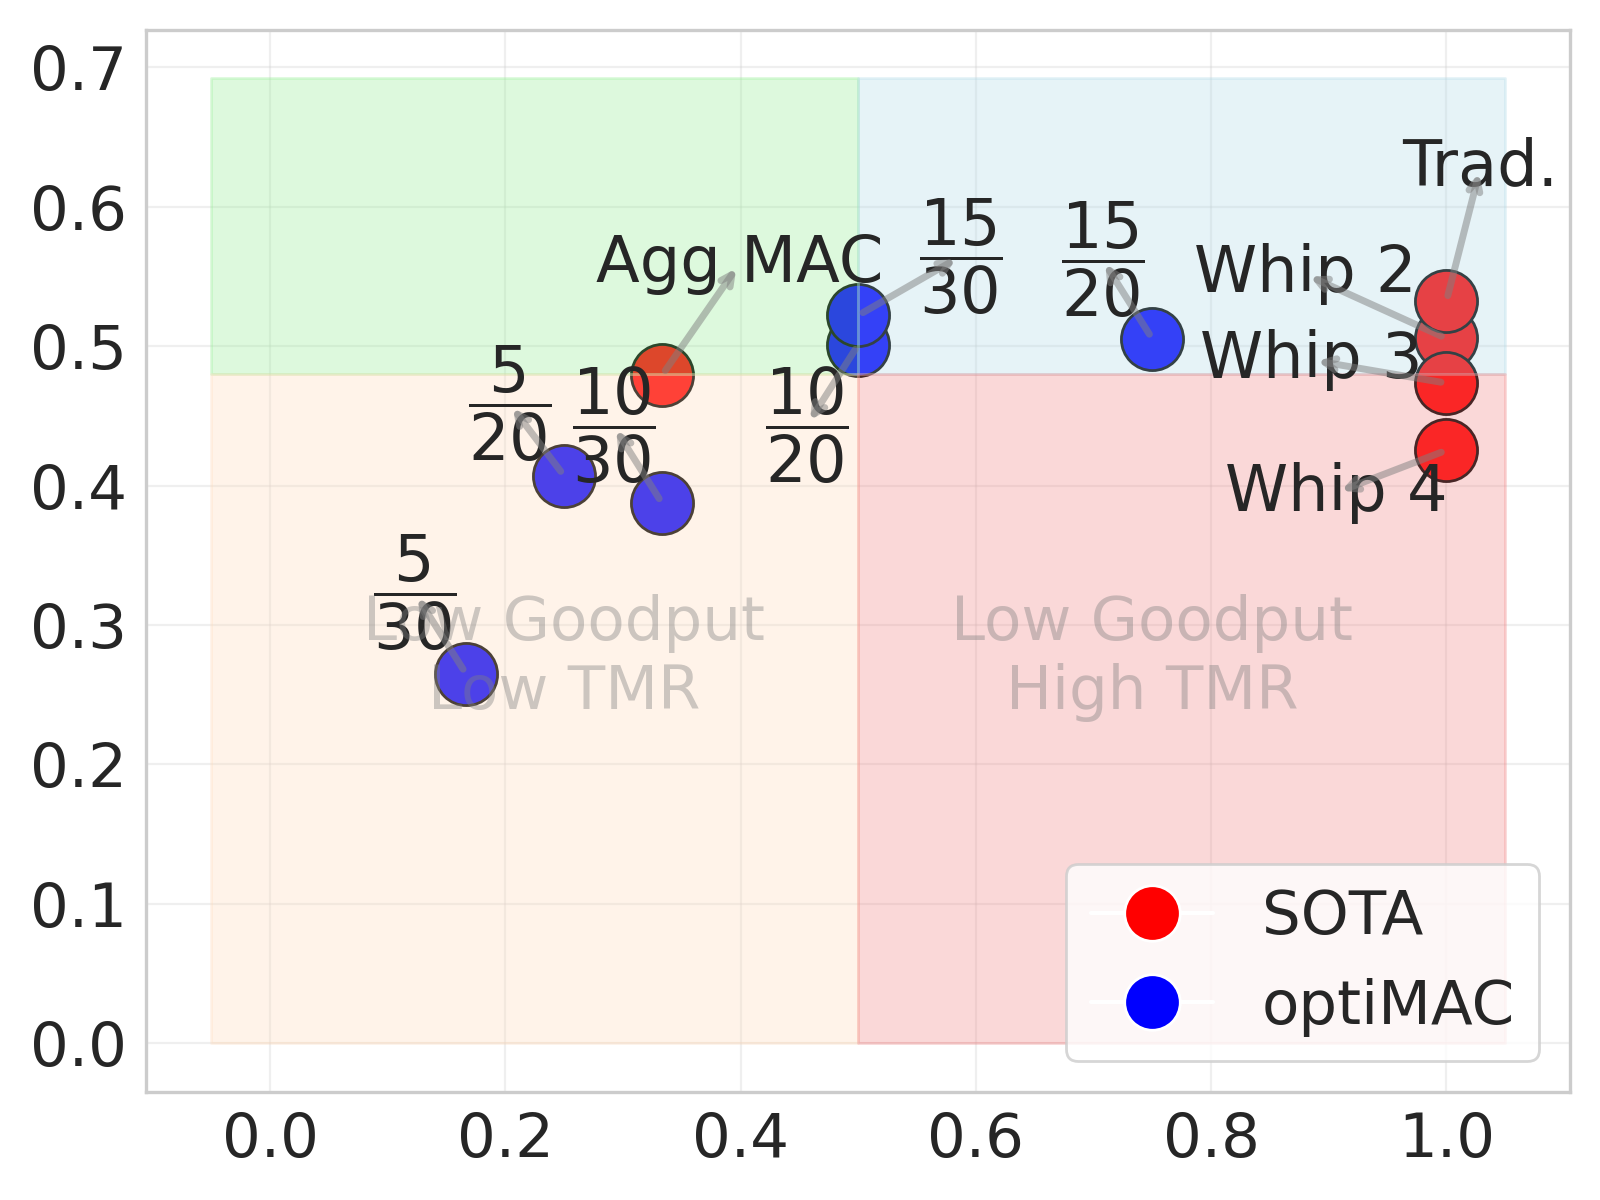
\includegraphics[width=\linewidth]{img/results/5G/0.2G'.png}
		\caption{Attack rate 0.2}
		\label{fig:0.2G 5G}
	\end{subfigure}
	\hfill
	\begin{subfigure}[b]{0.32\linewidth}
		\centering
		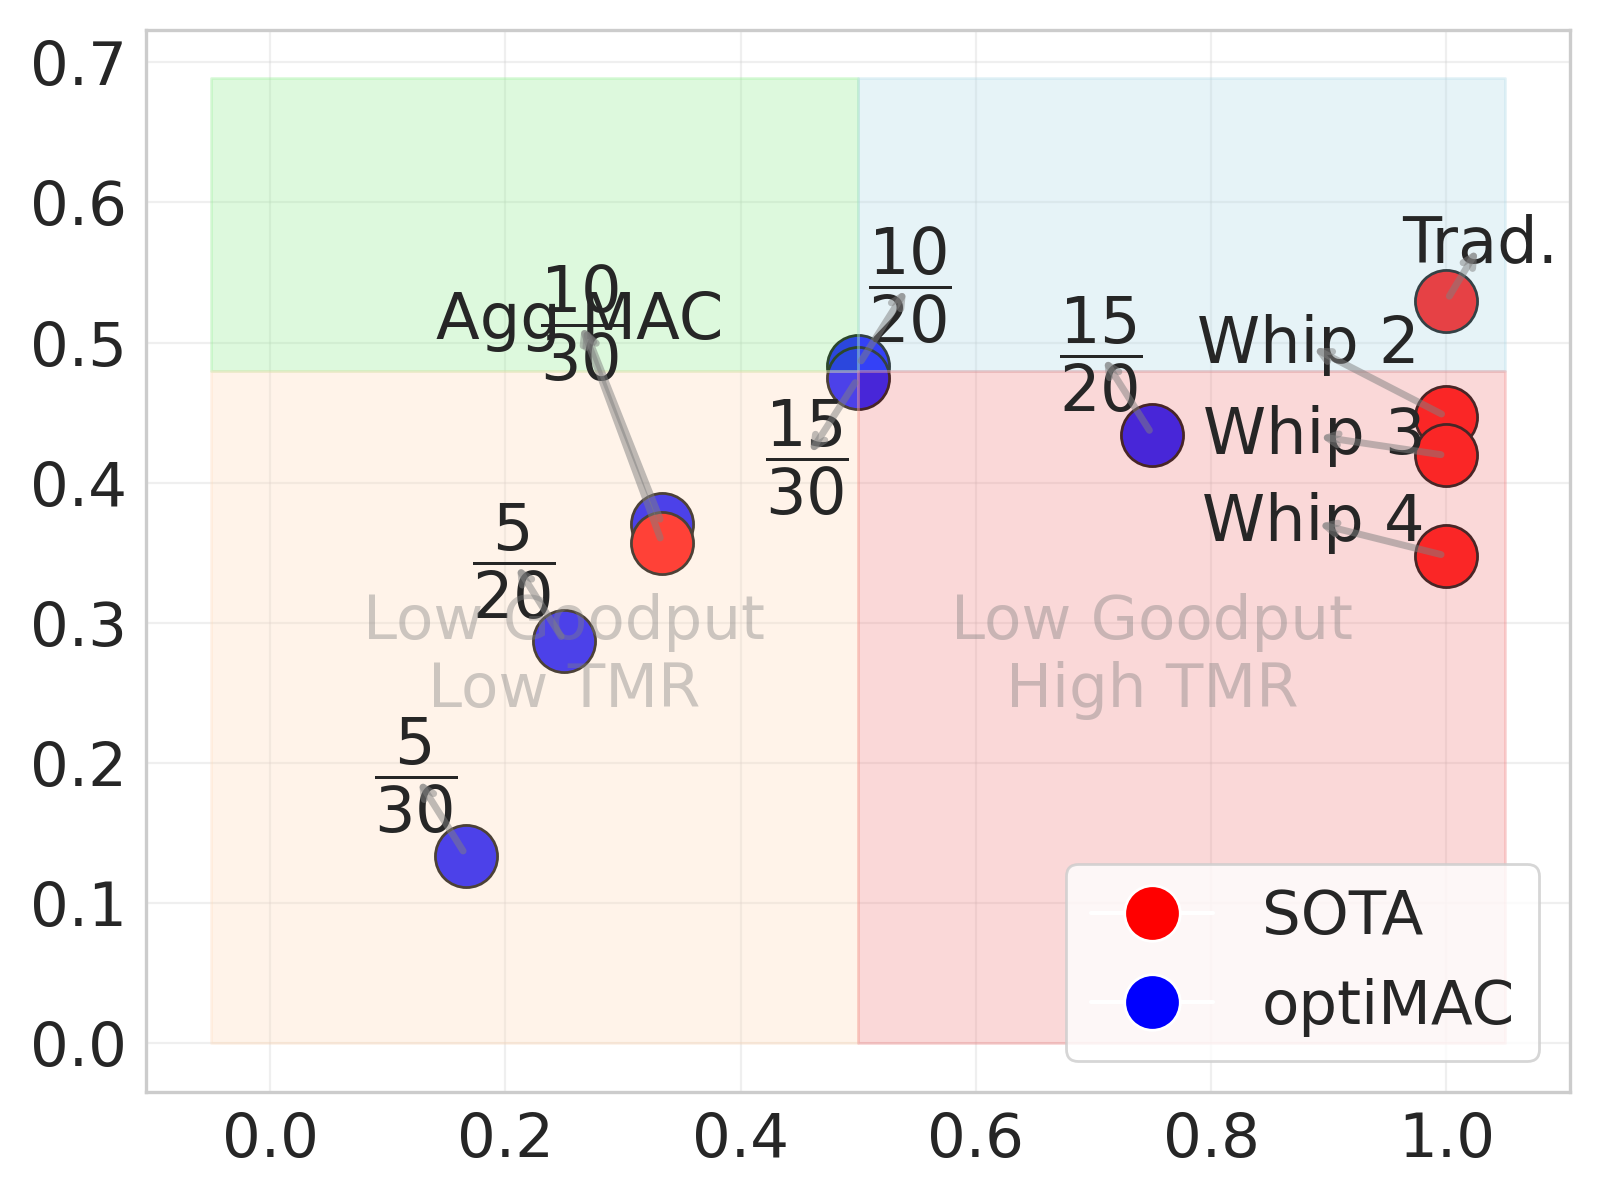
\includegraphics[width=\linewidth]{img/results/5G/0.3G'.png}
		\caption{Attack rate 0.3}
		\label{fig:0.3G 5G}
	\end{subfigure}
	
	\caption{Goodput (y-axis) vs. TMR (x-axis) of 5G experiments where more than 80\% of Traditional MAC's Goodput is considered high. State-of-the-art (SOTA) includes traditional, progressive, and aggregate MAC vs. the optiMAC.}
	\label{fig:goodput5G}
\end{figure*}

Figure~\ref{fig:Security5G} illustrates the performance of different MAC schemes (SOTA, OptiMAC, Agg. MAC, and various ProMAC versions) under varying attack rates (0.1, 0.2, and 0.3). Each subgraph plots the "Tag-bits per Message" (y-axis) against the "TMR" 
$\frac{n}{m}$ (x-axis), providing insights into the trade-offs between security and overhead.

We note that the WiFi results are not shown due to space limitations, as they exhibit trends nearly identical to the 5G results. Specifically, the relative performance ordering of the schemes, the security–overhead trade-offs, and the impact of increasing attack rates remain consistent across both network settings. Therefore, to avoid redundancy and improve clarity, we focus on presenting the 5G results, which are representative of both environments.

OptiMAC (depicted in blue) consistently achieves a balance between high security and low TMR, placing it in the "High Security, Low TMR" (green) region and satisfying Goal G2. It appears at lower tag-to-message ratios ($\frac{n}{m}$), indicating that it achieves strong security without requiring large redundancy, thereby reducing overhead. This demonstrates its efficiency compared to other schemes.

The SOTA solutions, shown in red, generally achieve high security but at higher TMR values, often placing them in the "High Security, High TMR" (blue) region, especially under higher attack rates. This indicates that while SOTA methods are effective, they incur significantly higher overhead compared to OptiMAC.

The Agg. MAC, when configured with a TMR of $\frac{1}{3}$, can achieve high security with low TMR under moderate attack rates, placing it in favorable regions of the plot. However, its performance degrades under higher attack rates (e.g., 0.3), where it transitions into the "Low Security, Low TMR" region, indicating insufficient robustness. In contrast, ProMAC variants (with dependency areas of 2, 3, and 4 without tag length adjustment) generally occupy the "Low Security, High TMR" or "High Security, High TMR" regions. While they can provide improved security over Agg. MAC, they do so at the cost of significantly increased overhead.

As the attack rate increases (from 0.1 to 0.3), all schemes exhibit a decrease in tag-bits per message, reflecting the need for increased redundancy to maintain security in more adversarial conditions.

Although not shown, the WiFi experiments follow the same trends, with differences in absolute values due to system parameters. In particular, WiFi exhibits lower tag-bits per message compared to 5G due to shorter tag lengths (32 vs. 64 bytes) and smaller payload sizes, as summarized in Table~\ref{tab:setting}.

Furthermore, by observing the trend of the OptiMAC configurations (blue points) in the goodput analysis (Figure~\ref{fig:goodput5G}), we identify a characteristic curve indicating an optimal operating region where goodput is maximized while maintaining required security levels (Goal G1). Selecting configurations near this peak enables an effective balance between security and efficiency under varying attack conditions.

\section{Conclusion}\label{Conclusion}
% Summarization of the research findings.
% Reflection on the impact and importance of the work in advancing IoT security.


% In this paper, we have introduced a comprehensive framework for analyzing and optimizing tag-to-message assignments in MAC techniques, addressing key challenges in secure communication systems, especially in lossy channel environments. By utilizing dependency graphs and matrices, we provided a systematic method for representing and analyzing the relationships between messages and tags. Our approach encompasses previous works as special cases, offering a more robust and flexible tool for studying MAC schemes.

% We defined and calculated critical metrics such as the authentication vector, latency vector, strength number, and security rate, providing a quantitative basis for assessing the robustness and efficiency of MAC schemes. Our framework leverages linear programming to optimize the expected number of authentication for various channel conditions, ensuring high security and reliability even in lossy environments.

% The results from our optimization demonstrate promising improvements in verification rates, and security. These improvements highlight the practical applicability of our theoretical advancements, providing a more secure and reliable solution for message authentication in lossy channels.

% Moreover, we discussed the potential for further enhancement of our framework through including the other metrics in the objective function. A different approach is to integrate of reinforcement learning. This adaptive approach could dynamically optimize the MAC schemes in real-time, providing even greater resilience and efficiency in variable network conditions.

% In conclusion, our research significantly advances the understanding and optimization of message authentication codes. The methodologies and metrics developed in this study lay a solid foundation for future research and practical applications, contributing to the development of more robust and efficient secure communication systems. We believe that our work will inspire further innovations in this critical area of network security.

This work presents OptiMAC, a framework for optimizing integrity verification in lossy and adversarial communication channels. OptiMAC addresses the trade-off between security and efficiency in MAC schemes by introducing a dependency-graph representation and a mixed-integer linear programming formulation for tag-to-message assignment. 

Unlike traditional and heuristic-based approaches, OptiMAC moves beyond fixed or ad hoc configurations. While ProMAC established a general framework, it did not provide a systematic method for determining key parameters such as tag generation, update rules, and assignment strategies. OptiMAC fills this gap by modeling assignments as a dependency graph and optimizing them mathematically, ensuring configurations are tailored to the operating environment.

Evaluations in WiFi and 5G scenarios show that OptiMAC achieves higher effective security while operating at lower tag-to-message ratios than prior schemes. These results demonstrate the framework’s practicality for energy-sensitive and mission-critical applications, where efficiency and robustness must coexist.

% Looking ahead, this foundation enables further research into adaptive
% techniques that jointly optimize latency, efficiency, and security. A promising
% direction is the development of real-time models that adjust tag-to-message
% configurations dynamically in response to changing channel conditions. Such
% extensions would push OptiMAC toward delivering even stronger guarantees for
% the evolving demands of secure wireless communication.






\bibliographystyle{plain}
\bibliography{references}

\end{document}
